%!TEX root = ../thesis.tex
%*******************************************************************************
%*********************************** First Chapter *****************************
%*******************************************************************************

\chapter{Results}  %Title of the First Chapter
\label{chapterresults}

\ifpdf
\graphicspath{{Chapter5/Figs/Raster/}{Chapter5/Figs/PDF/}{Chapter5/Figs/}}
\else
\graphicspath{{Chapter5/Figs/Vector/}{Chapter5/Figs/}}
\fi

One of the aims of this study was to check how the designed impedance device detects plethysmography signals. Another objective was to verify how what changes in plethysmography waveform are detectable by the instrument. As described in chapter \ref{chapterdesign} the designed device is capable of providing electrical signals comparable to the impedance of the body section. The iPG instrument provides output ports of the current driven into the patient, impedance readings and plethysmography waveform of volume under test. In chapter \ref{chapterprocedure}, these signals were converted from voltage representations into readable units such as impedance values in ohms (\si{\ohm}) and currents (\si{\ampere}). Then, a GUI provided analysis of the signals, as well as post-processing options. Last, the data was converted into measurements of blood flow.

As it was described in chapter \ref{chapterprocedure}, the experiment proceeds by recording five minutes of baseline signal followed by a level of occlusion. According to this, seven different regions are identifiable in the experiment, as presented on Table \ref{tbl:Z_regions}. Also, occlusive events are represented as shaded areas in figure \ref{fig:rb:all_participants}. Regions 1, 3, 5 and 7 refer to the five minutes of baseline waveform. On the other hand, regions 2, 4 and 6 are equivalent to venous, partial arterial and total occlusions.

This chapter describes the results obtained from the experimental work. It will show the device capability of detecting impedance baseline signals and plethysmography waveforms. Later, an outline of the numeric results during occlusion will be explained when compared to the additional instruments used during the study. 

\mynote{First report the volume measured and the impedance correlated}


%%********************************** % Section 5.1 ******************************************
\section{Physiological measurements}
\label{section5.1}
In the beginning of the research, from the participants recruited population characteristics, physiological measurements and blood pressure values were taken \mynote{reference to section that includes a figure of the arm with the measurements position}. In total three female and six male took part of the study. Their age were between \SIrange{23}{37}{year-old} (mean $29.12 \pm 4.94$). The table \ref{tbl:physiological} overviews the data and measurements collected from the participants previous the experiment.

\begin{table}[htbp] %tbl:physiologica
	\caption{Participants' forearm measurements and initial volume.}
	\label{tbl:physiological}
	\centering
	\begin{tabular}{lcc|ccc}
		\toprule
		&              &              &         \multicolumn{3}{c}{\textbf{Dimensions [\si{\cm}]}}         \\
		& \textbf{Age} & \textbf{Sex} & \textbf{Arm length} & \textbf{Shoulder} & \textbf{Total length} \\
		&              &              &                     &  \textbf{to heart}   &                       \\ \midrule
		Participant 1 &      26      &     Male     &         80          &          26          &          106          \\
		Participant 2 &      23      &    Female    &         66          &          24          &          90           \\
		Participant 3 &      27      &    Female    &         74          &          24          &          98           \\
		Participant 4 &      37      &     Male     &         68          &          24          &          92           \\
		Participant 5 &      29      &    Female    &         62          &          24          &          86           \\
		Participant 6 &      36      &     Male     &         70          &          24          &          94           \\
		Participant 7 &      29      &     Male     &         73          &          23          &          96           \\
		Participant 8 &      26      &     Male     &         69          &          23          &          92           \\ \bottomrule
	\end{tabular}
\end{table}

From the sensing electrodes position is possible to estimate the segment's volume by measuring the distance between electrodes ($l$), circumference of each electrode (C$_1$ and C$_2$).  This measuring method is not very accurate (see section \mynote{Add reference to a section where how measurements were taken}) but at least guesses a picture of the initial volume of the conductive segment. Table \ref{tbl:measurments} shows the dimensions of the participants forearm between the sensing electrodes and the segment's volume calculate from Equation \ref{eq:v_e}.

\begin{table}[htbp] %tbl:measurments
	\caption{Participants' forearm measurements and initial volume.}
	\label{tbl:measurments}
	\sisetup{separate-uncertainty=true}
	\centering
	\begin{tabular}{lcccccc    S[table-format=2.2]@{\,\( \pm \)\,}S[table-format=1.2]}
		\toprule
		&  \textbf{L [\si{\cm}]}   &  \textbf{C$_1$ [\si{\cm}]}  &  \textbf{C$_2$ [\si{\cm}]}  &   \textbf{Ve [\si{\cubic\cm}]} \\\midrule
		Participant 1 & 14.8 & 17.5 & 27.5 & 606.05 \\
		Participant 2 & 11.0 & 15.0 & 20.0 & 269.90 \\
		Participant 3 & 13.0 & 19.0 & 26.5 & 540.27 \\
		Participant 4 & 10.0 & 17.5 & 25.0 & 363.07 \\
		Participant 5 & 10.0 & 17.5 & 23.5 & 336.81 \\
		Participant 6 & 11.0 & 18.5 & 27.0 & 458.32 \\
		Participant 7 & 13.5 & 15.0 & 23.0 & 393.55 \\
		Participant 8 & 11.5 & 17.0 & 23.5 & 378.49 \\ \bottomrule
	\end{tabular}
\end{table}

Executing a mechanical occlusion of the upper arm limits the blood flow towards the forearm. As detailed in the chapter  \ref{chapterprocedure}, blood pressure was taken before the study began. The mean systolic and diastolic pressures were \SI{116.25}{\mmHg}$\pm$\SI{13.66}{\mmHg} and \SI{72.75}{\mmHg}$\pm$\SI{7.23}{\mmHg} respectively. Venous occlusion took place below systolic pressure (mean \SI{55}{\mmHg}$\pm$\SI{8.01}{\mmHg}), partial arterial pressure calculated from equation \ref{eq:meanpressure} was about  \SI{94.63}{\mmHg}$\pm$\SI{10.21}{\mmHg} and total occlusion was around \SI{136.25}{\mmHg}$\pm$\SI{13.67}{\mmHg}. Table \ref{tbl:occlusions} details the blood pressures recorded.

\begin{table}[htbp] %tbl:occlusions
	\caption{Participants' initial blood pressure and levels for venous, partial arterial and total occlusion.}
	\label{tbl:occlusions}
	\centering
	\begin{tabular}    {lcccc}
		\toprule
		& \textbf{Blood pressure}  &  \textbf{Occlusion 1}   & \textbf{Occlusion 2}  &  \textbf{Occlusion 3} \\
		&  [\si{\mmHg}]   &        [\si{\mmHg}]  &    [\si{\mmHg}]   &  [\si{\mmHg}]\\ \midrule
		Participant 1  &  124/78   &        50  &    101   &  144\\ 
		Participant 2  &  105/65   &        50  &     85   &  125 \\
		Participant 3  &  120/78   &        60  &     99   &  140 \\
		Participant 4  &  120/72   &        60  &     96   &  140 \\
		Participant 5  &  100/60   &        40  &     80   &  120 \\
		Participant 6  &  143/82   &        60  &    113   &  163 \\
		Participant 7  &  107/73   &        65  &     90   &  127 \\
		Participant 8  &  111/74   &        55  &     93   &  131 \\\bottomrule
	\end{tabular}
\end{table}


%%********************************** % Section 5.2 ******************************************
\section{Impedance results from mean resistivity value}
\label{section5.2}
As described in the previous chapters\mynote{Maybe add a reference of the past chapter design of the device}, the iPG device provides an output signal denominated $Z_{DC}$ which is equivalent to the mean impedance value of the elbow to wrist section. Moreover, it includes an AC component equal to a low-resolution plethysmography signal. However, this waveform at this point is unwanted, but it will be helpful for analysis beat by beat. This section will analyse the changes that the impedance baseline suffer during the different events of the experiment.

The resistivity mean value is known as basal impedance, which it is equivalent to the value $R_B$ described by Nyober's equation \ref{eq:Nyober} or the foot of the signal in the plethysmography waveform. In other words, it is the value of the impedance before circulation occurs. It is composed basically of the impedance contribution of bone, muscle, fat, skin and residual blood within the vessels.

\mynote{Maybe add a waveform explaining where the signal was extracted form or from a reference to another section}

As explained in detail in chapter \ref{chapterprocedure}, the experimental protocol required executing a mechanical compression using a cuff to limit venous and arterial blood inflow and outflow. The pressures level of these occlusions have been recorded in table \ref{tbl:occlusions}. First, venous blockage causes a swelling of the forearm by filling of the capillaries below the blockage. Second, during partial arterial occlusion, the incoming arterial flow is restricted causing a slow filling of the forearm's vessels. In both kinds of occlusions, the blood pooling increases the volume of the forearm's segment, hence producing a variation in the baseline signal. In contrast, total occlusion completely eliminates the blood inflow under the obstructed section; it is a tourniquet effect. Thus, the resultant impedance should be similar to the baseline resistivity.

Analysing the baseline requires eliminating the waveform component of the signal. In section \mynote{Add a section in data processing explaining how the value of $R_B$ was extracted for this analysis and reference it.} was explained in detail the steps required to obtained this level of the signal. In the end, only the values from the foot of the signal equivalent to $R_B$ were extracted. Figure \ref{fig:rb:all_participants} shows all the basal impedance signals of all the participants during the whole study. As can be seen, some signals were affected by motion artefact. In fact, other instruments such as PPG and ultrasound Doppler also picked up these sort of fluctuations. Table \ref{tbl:Z_regions} shows the mean value of the impedance separated in regions or events. In the following sections, the changes in basal impedance will be analysed more in depth. 

\begin{sidewaystable}[htbp] %tbl:Z_regions
	\caption{Mean basal impedance divided in seven regions}
	\label{tbl:Z_regions}
	\centering
	\begin{tabular}    {l
			*{7}{S[table-format=2.2]@{\,\( \pm \)\,}S[table-format=1.2]} %Format for Z+-std
		}
		\toprule
		&\multicolumn{2}{c}{\textbf{Region 1}}&\multicolumn{2}{c}{\textbf{Region 2}}&\multicolumn{2}{c}{\textbf{Region 3}}&\multicolumn{2}{c}{\textbf{Region 4}}&\multicolumn{2}{c}{\textbf{Region 5}}&\multicolumn{2}{c}{\textbf{Region 6}}&\multicolumn{2}{c}{\textbf{Region 7}}\\
		&\multicolumn{2}{c}{\small{\SIrange{0}{300}{\second}}}&\multicolumn{2}{c}{\small{\SIrange{300}{480}{\second}}}&\multicolumn{2}{c}{\small{\SIrange{480}{780}{\second}}}&\multicolumn{2}{c}{\small{\SIrange{780}{960}{\second}}}&\multicolumn{2}{c}{\small{\SIrange{960}{1260}{\second}}}&\multicolumn{2}{c}{\small{\SIrange{1260}{1440}{\second}}}&\multicolumn{2}{c}{\small{\SIrange{1440}{1740}{\second}}} \\                                   &\multicolumn{2}{c}{$\bar{\textrm{Z}}$ [\si{\ohm}]}&\multicolumn{2}{c}{$\bar{\textrm{Z}}$ [\si{\ohm}]}&\multicolumn{2}{c}{$\bar{\textrm{Z}}$ [\si{\ohm}]}&\multicolumn{2}{c}{$\bar{\textrm{Z}}$ [\si{\ohm}]}&\multicolumn{2}{c}{$\bar{\textrm{Z}}$ [\si{\ohm}]}&\multicolumn{2}{c}{$\bar{\textrm{Z}}$ [\si{\ohm}]}&\multicolumn{2}{c}{$\bar{\textrm{Z}}$ [\si{\ohm}]}\\\midrule
		Participant 1  &  77.59  &    0.17  &  77.24   &   0.14  &  77.67  &    0.16   & 76.73  &    0.48  &  76.84   &   0.79  &  76.64  &    0.28  &  76.61   &   0.22\\
		Participant 2  &  96.97  &    0.09  &  96.54   &   0.22  &  97.15  &    0.23   & 96.52  &    0.37  &  97.01   &   0.18  &  97.15  &    0.07  &  97.50   &   0.13\\
		Participant 3  &  93.54  &    0.50  &  93.37   &   0.23  &  93.08  &    0.94   & 93.04  &    0.34  &  92.21   &   0.30  &  92.14  &    0.30  &  91.43   &   0.85\\
		Participant 4  &  63.44  &    0.19  &  62.80   &   0.16  &  62.40  &    0.24   & 62.21  &    0.25  &  62.47   &   0.54  &  63.37  &    0.13  &  66.03   &   6.47\\
		Participant 5  &  69.97  &    0.17  &  69.60   &   0.23  &  69.77  &    0.16   & 69.23  &    0.41  &  68.99   &   0.13  &  69.02  &    0.04  &  69.21   &   0.21\\
		Participant 6  &  57.68  &    0.17  &  57.63   &   0.08  &  57.77  &    0.11   & 57.35  &    0.20  &  57.31   &   0.19  &  57.08  &    0.07  &  57.22   &   0.41\\
		Participant 7  &  94.72  &    0.24  &  93.75   &   0.23  &  93.46  &    0.28   & 92.37  &    0.26  &  92.63   &   0.11  &  92.87  &    0.17  &  92.57   &   0.10\\
		Participant 8  &  80.04  &    0.11  &  79.75   &   0.10  &  79.85  &    0.11   & 79.23  &    0.25  &  79.24   &   0.21  &  78.87  &    0.05  &  78.60   &   0.11\\\bottomrule
	\end{tabular}
\end{sidewaystable}

\begin{figure}[htbp]  %fig:rb:all_participants
	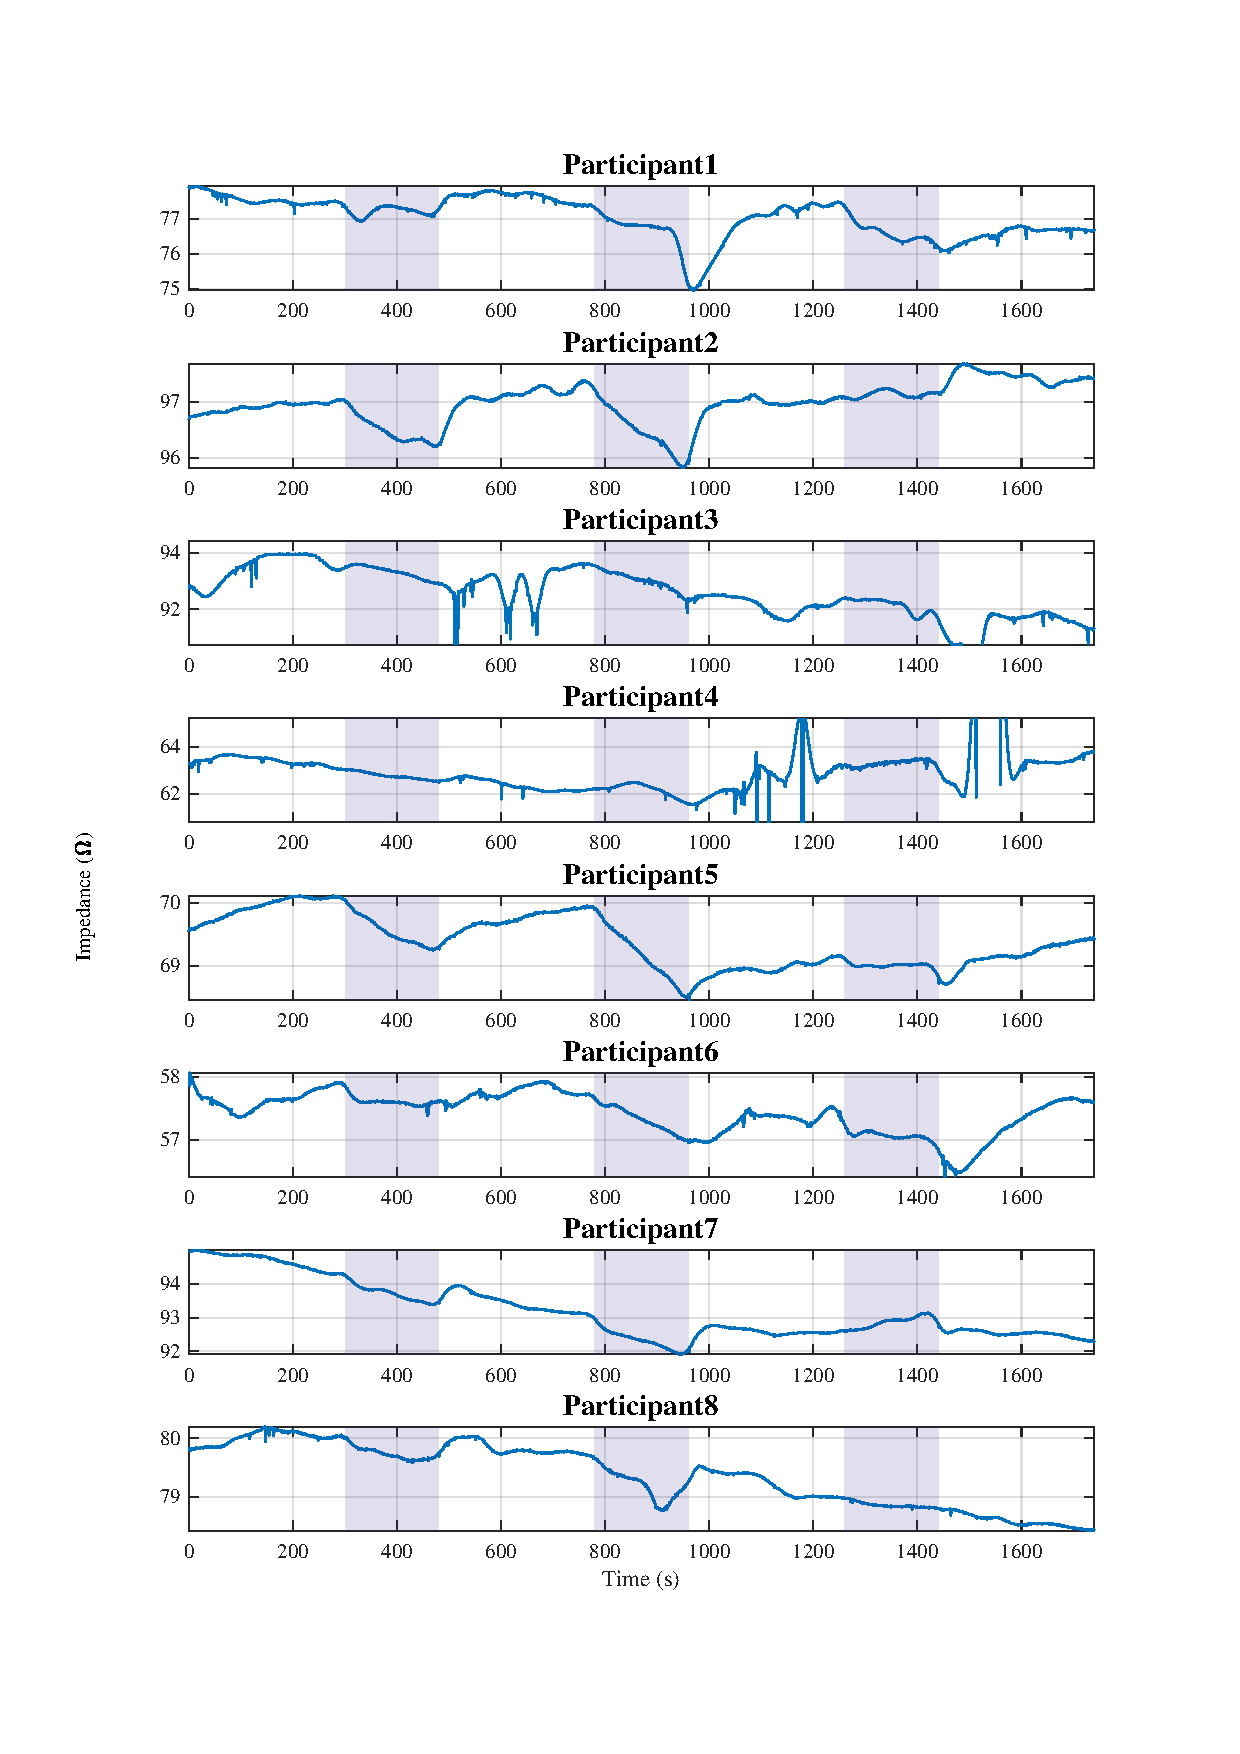
\includegraphics[width=\textwidth,height=\textheight,keepaspectratio]{figure1}    
	\caption{Baseline impedance of all the participants during the study. The shaded areas represent occlusions events.}
	\label{fig:rb:all_participants}
\end{figure}
\mynote{This figure is temporary. It needs to be improved by naming axis}

%%********************************** % Section 5.2.1 ******************************************
\subsection{Baseline impedance}
\label{section5.2.1}
The iPG device recorded the impedance during the first five minutes of data logging. The device was able to detect the forearm's segment impedance quite remarkably. The values obtained felt within the resistive value estimated by the literature \mynote{Find some papers with results about the impedance of the forearms}. The table \ref{tbl:basal_impedace:region1} describes the basal impedance during the first five minutes of data. 

\begin{table}
	\caption{Basal impedance during the first five minutes of data with statistical values.}
	\label{tbl:basal_impedace:region1}
	
	\centering
	\begin{tabular}        
		{
			l
			c
			S[table-format=2.2]@{\,\( \pm \)\,}S[table-format=1.2] %Format for Z+-std
			*{2}{S[table-format=2.2]} 
		}
		\toprule
		& \textbf{Size} & \multicolumn{2}{c}{\textbf{ $\bar{\textrm{Z}}$ [\si{\ohm}]}} & \textbf{Max [\si{\ohm}]} & \textbf{Min [\si{\ohm}]} \\ \midrule
		Participant 1  &  278  &  77.59  &  0.17  &  78.04  &  77.37\\
		Participant 2  &  295  &  96.97  &  0.09  &  97.17  &  96.76\\
		Participant 3  &  275  &  93.54  &  0.50  &  94.06  &  92.44\\
		Participant 4  &  329  &  63.44  &  0.19  &  63.77  &  63.02\\
		Participant 5  &  288  &  69.97  &  0.17  &  70.20  &  69.56\\
		Participant 6  &  331  &  57.68  &  0.17  &  58.21  &  57.33\\
		Participant 7  &  340  &  94.72  &  0.24  &  95.05  &  94.27\\
		Participant 8  &  353  &  80.04  &  0.11  &  80.30  &  79.82\\ \bottomrule
	\end{tabular} 
\end{table} 

There are different aspects of the geometry that could affect the impedance reading. There have been several studies where has been demonstrated how the distance between electrodes affects readings\mynote{Add reference to studies impedance vs. length}. In the current study showed that impedance was influenced by the forearm's circumference, as well as the distance between the potential electrodes. Figure \ref{fig:C_vs_Z} indicates that there is an inverse relation between circumference and impedance. The smallest the forearm's circumference higher the resistivity. On the other hand, there is a direct relation between the distance between the potential electrodes and the resistivity of the segment as depicted in \ref{fig:l_vs_Z}.

In contrast, when comparing total volume measured and mean resistivity of the segment, there is a slight drop of impedance, but it is not a clear tendency (see figure \ref{fig:Ve_vs_Z}). As it can be noticed, the data points are scattered depicting a not clear trend. This lack of bias can be explained as the fat content can affect impedance measurements. As explained by xxx \mynote{Add reference about the affinity of fat and impedance}, fat is a good conductor of electricity. Hence, fat content does not allow to show a clear tendency in impedance and volume. Nevertheless, in the end, the change of volume from the first basal impedance is going to be caused by the blood streaming trough the vessels.  

\begin{figure*}[t!]
	\centering
	\begin{subfigure}[t]{0.5\textwidth}
		\centering
		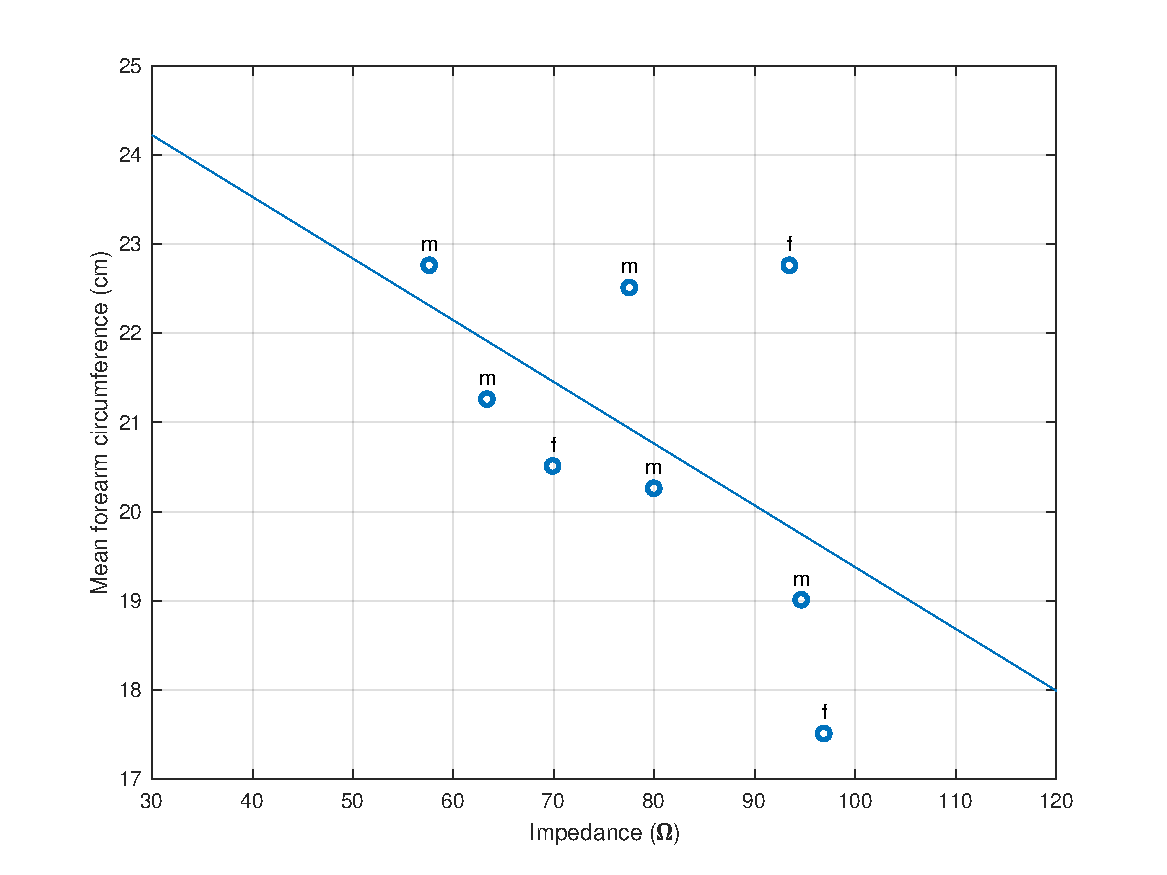
\includegraphics[height=6cm]{figure2a}
		\caption{Relationship between forearm circumference and mean basal impedance}
		\label{fig:C_vs_Z}
	\end{subfigure}%
	~ 
	\begin{subfigure}[t]{0.5\textwidth}
		\centering
		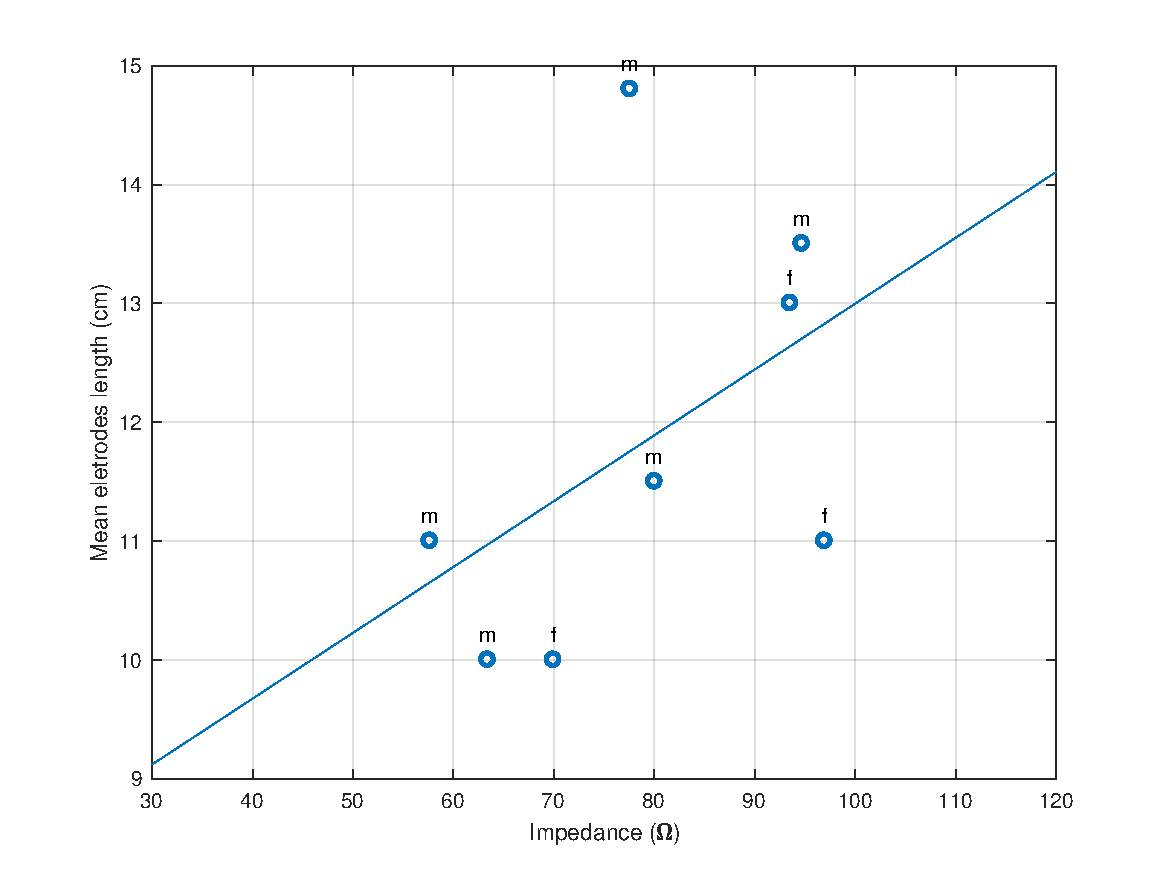
\includegraphics[height=6cm]{figure2b}
		\caption{Relationship between distance sensing electrodes and mean basal impedance}
		\label{fig:l_vs_Z}
	\end{subfigure}
	~ 
	\begin{subfigure}[t]{0.5\textwidth}
		\centering
		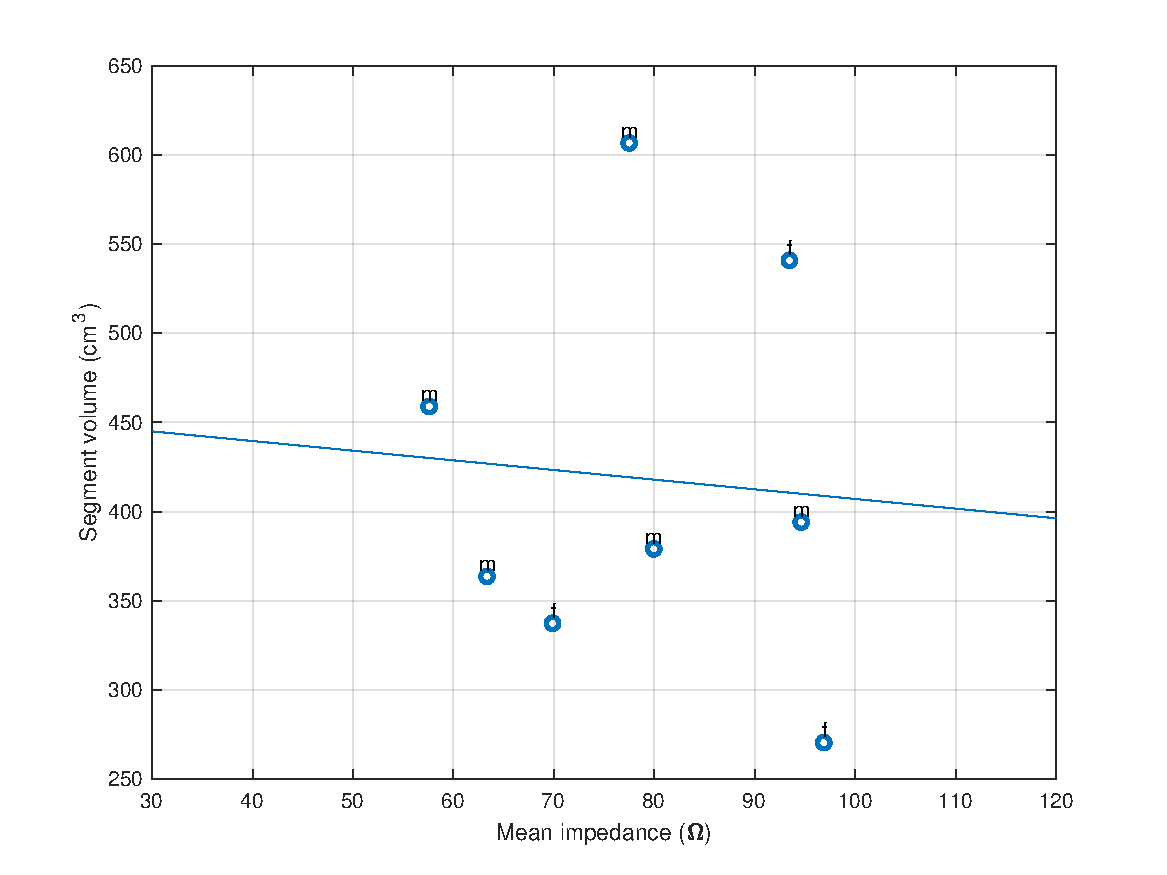
\includegraphics[height=6cm]{figure2c}
		\caption{Relation between forearms segment volume and mean basal resistivity}
		\label{fig:Ve_vs_Z}
	\end{subfigure}
	\caption{Relation between circumference, length and total segment's volume and mean basal impedance}
	\label{fig:relation_geometry_vs_impedance}
\end{figure*}


%%********************************** % Section 5.2.2 ******************************************
\subsection{Mean impedance measurement during venous occlusion}
\label{section5.2.2}
During the following three minutes after the impedance, venous occlusion occurred. As it can be seen in figure \ref{fig:rb:all_participants} all the participants experienced a decrease in basal impedance during this time. Most of the helpers presented a linear impedance decrease trend during the occlusion. However, some of the measurements were clearly affected by motion artefact. Participants one and six are an example of this. 

In participant one, resistance fell off immediately the occlusion occurred. Nevertheless, after a minute the patron moved his arm correcting the trend. Then, impedance continued the trend again. Furthermore,  participant six also showed similar response when the arm moved. 

Figure \ref{fig:normalise:venous_occlusion} describes how the impedance behaved during the occlusion for all participants. The graph has been normalised to compare the resistivity reduction.  A linear regression was performed in the data to demonstrate the ratio of change during the occlusion.  

The table \ref{tbl:venous_occlusion:region2} overviews the results obtained from the linear regression. The value $Z_1$ illustrates the value of the impedance as the blockage started and $Z_{end}$ the resistance value at the end of the test.  $\Delta Z$ (mean $-0.632 \Omega \pm0.068\Omega$) is the variation of impedance during the \SI{3}{\minute} that the experiment last.  The slope demonstrates how much resistance is changing during each beat  (mean $-0.00271\Omega\textrm{/s}\pm3.415e^{-6}\Omega\textrm{/s}$). 

\begin{figure}
	\centering
	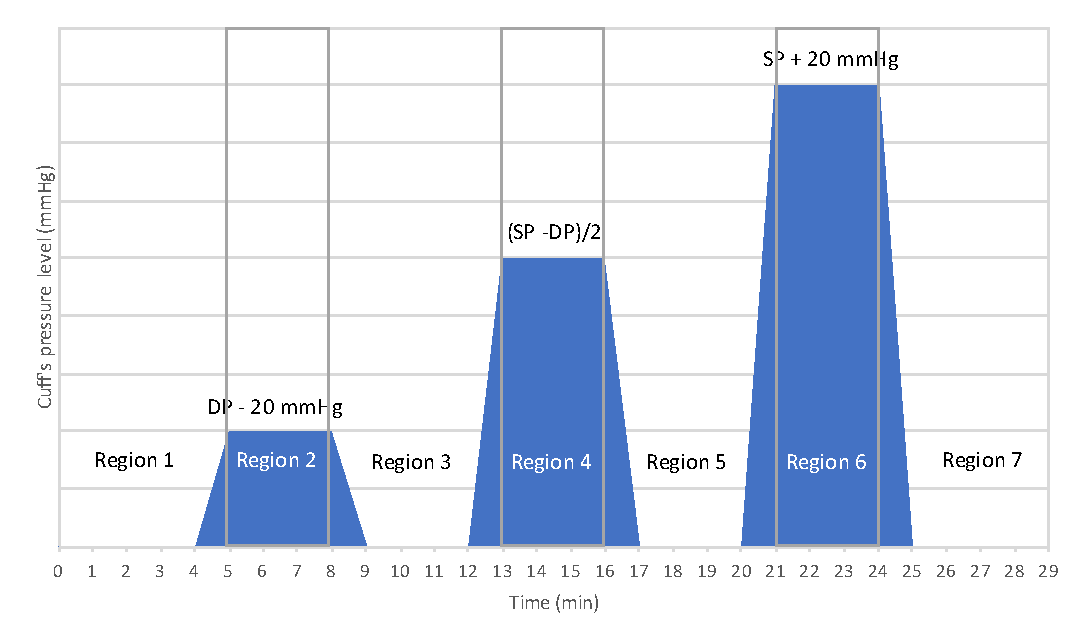
\includegraphics[width=0.9\textwidth,height=0.9\textheight,keepaspectratio]{figure3}    
	\caption{Normalise plot of impedance decrease during venous occlusion.}
	\label{fig:normalise:venous_occlusion}
\end{figure}
\mynote{Figure \ref{fig:normalise:venous_occlusion} is temporary. It needs to be improved by naming axis}

\begin{table}[htbp]
	\caption{Linear regression result for all participants during venous occlusion.}
	\label{tbl:venous_occlusion:region2}
	\centering
	\begin{tabu}{lcccccc}
		\toprule
		& \textbf{Slope [\si{\ohm/\second}]} & \textbf{Intercept [\si{\ohm}]} & \textbf{$R^2$} & \textbf{$Z_1$ [\si{\ohm}]} & \textbf{$Z_{end}$ [\si{\ohm}]} & \textbf{ $\Delta Z$ [\si{\ohm}]} \\ \midrule
		Participant 1  &   0.00057  &  77.02   &     0.037  &  77.49  &  77.18  &  -0.31\\
		Participant 2  &  -0.00395  &  98.09   &     0.867  &  97.16  &  96.21  &  -0.95\\
		Participant 3  &  -0.00421  &  95.01   &     0.917  &  93.47  &  92.89  &  -0.58\\
		Participant 4  &  -0.00296  &  63.96   &     0.920  &  63.22  &  62.61  &  -0.61\\
		Participant 5  &  -0.00427  &  71.26   &     0.936  &  70.10  &  69.27  &  -0.83\\
		Participant 6  &  -0.00085  &  57.96   &     0.322  &  57.98  &  57.57  &  -0.40\\
		Participant 7  &  -0.00427  &  95.42   &     0.934  &  94.33  &  93.34  &  -0.98\\
		Participant 8  &  -0.00173  &  80.43   &     0.752  &  80.07  &  79.68  &  -0.39\\ \bottomrule
	\end{tabu} 
\end{table}

From the statistical analysis displayed can be concluded the following. First, as it was explained before, the slopes from participants 1 and 6 were affected by the motion artefact. Nevertheless, these trends seemed corrected after one minute of recordings (\SI{360}{\second}). Their slopes were quite far away from the mean value (\SI{-0.00271}{\ohm\per\second}$\pm$\SI{3.415e-06}{\ohm\per\second}). On the other hand, the rest of the signals showed a similar trend. \mynote{Review this paragraph. It seems to be very similar to the previous one.}


%%********************************** % Section 5.2.3 ******************************************
\subsection{Mean impedance data during arterial occlusion}
\label{section5.2.3}
During partial arterial occlusion (\SIrange{480}{760}{\second}), the incoming arterial flow is restricted causing a slow filling of the forearm. This mechanical blocking induces an uncomfortable feeling to the participants, some of them felt numbness in the arm.  As it can be seen from figure \ref{fig:rb:all_participants}, most of the participants there is an apparent drop in impedance during the action. Though participant one moved his muscles creating a sharp fall before releasing the pressure, also partaker four showed a slight increment of impedance followed in the middle of this part of the test. 

Figure \ref{fig:normalise:arterial_occlusion} shows the normalise resistivity decrease for all the participants. Table \ref{tbl:arterial_occlusion:region4} shows the values of the linear regression for the data.   All in all, it is clear that the decrease of resistivity is sharper in this part of the experiment compared to venous occlusion.  In fact, when this data is compared to venous information, the average slope is nearly twice as big (mean \SI{-0.00536}{\ohm\per\second}$\pm$\SI{2.853e-06}{\ohm\per\second}). Also, the total change of impedance ($\Delta Z$) was almost doubled in all participants, except participant four which value decreased.  

The linear regression of this region of the signal showed an apparent straight tendency for most of the participants. Most of the signals can be represented as negative tilt line ($R^2 \geq 0.858 $), except members one, four and eight ($R^2 \leq 0.627 $).

\mynote{Check about what happens during partial arterial occlusion. Slow filling of the forearm. This information should also be added to the Medical Background}
\begin{figure}
	\centering
	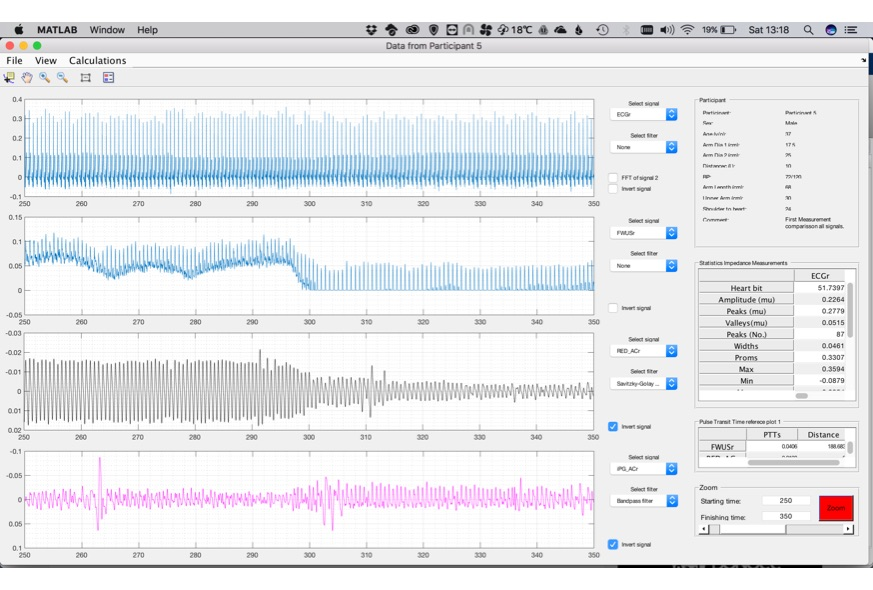
\includegraphics[width=0.9\textwidth,height=0.9\textheight,keepaspectratio]{figure4}    
	\caption{Normalise plot of impedance decrease during partial arterial occlusion.}
	\label{fig:normalise:arterial_occlusion}
\end{figure}
\mynote{Figure \ref{fig:normalise:venous_occlusion} is temporary. It needs to be improved by naming axis}

\begin{table}[htbp]
	\caption{Linear regression result for all participants during partial arterial occlusion.}
	\label{tbl:arterial_occlusion:region4}
	\centering
	\begin{tabu}{lcccccc}
		\toprule
		& \textbf{Slope [\si{\ohm/\second}]} & \textbf{Intercept [\si{\ohm}]} & \textbf{$R^2$} & \textbf{$Z_1$ [\si{\ohm}]} & \textbf{$Z_{end}$ [\si{\ohm}]} & \textbf{ $\Delta Z$ [\si{\ohm}]} \\ \midrule
		Participant 1  &  -0.00656  &   82.44    &   0.519  &  77.51  &  74.91  &  -2.60 \\
		Participant 2  &  -0.00706  &  102.67    &   0.965  &  97.29  &  95.75  &  -1.54 \\
		Participant 3  &  -0.00601  &   98.28    &   0.858  &  93.61  &  92.20  &  -1.41 \\
		Participant 4  &  -0.00327  &   65.05    &   0.474  &  62.25  &  61.81  &  -0.44\\
		Participant 5  &  -0.00767  &   75.89    &   0.989  &  70.05  &  68.50  &  -1.55\\
		Participant 6  &  -0.00366  &   60.53    &   0.939  &  57.74  &  56.88  &  -0.85\\
		Participant 7  &  -0.00490  &   96.64    &   0.969  &  93.11  &  92.02  &  -1.09\\
		Participant 8  &  -0.00381  &   82.54    &   0.627  &  79.70  &  79.10  &  -0.59\\ \bottomrule
	\end{tabu} 
\end{table}



%%********************************** % Section 5.2.4 ******************************************
\subsection{Mean impedance data during total occlusion}
\label{section5.2.4}
Producing a total occlusion (between \SIrange{1260}{1440}{\second}) in the upper arm stops the blood inflow completely under the obstructed section. This test caused much discomfort on most of the participants, which made them moving their limbs voluntary. Because there is no blood pooling during this part of the experiment is expected not seeing a common tendency in impedance variation. Additionally, the mean restive value is equivalent to the impedance of the tissue components within the segment plus the impedance of the residual blood in the forearm. However, when a change of resistivity happens is mostly caused by the participant's re-accommodation rather than a physiological variable. 

After analysing the data obtained (see  Table \ref{tbl:total_occlusion:region6} and figure \ref{fig:normalise:total_occlusion}), it can be noticed that there is not a defined trend for most of the signals. The slopes and deltas computed show a variation between negative and positive values. Therefore, it can be concluded that there is not an indication of a clear bias common to the signals. 

The impedance plethysmography signal can confirm the absence of blood flow. On section xxx \mynote{Add reference in plethysmography that shows the waveforms} is shown the lack of peaks in the signal. 

\mynote{Check about what happens during partial arterial occlusion. Slow filling of the forearm. This information should also be added to the Medical Background}
\begin{figure}
	\centering
	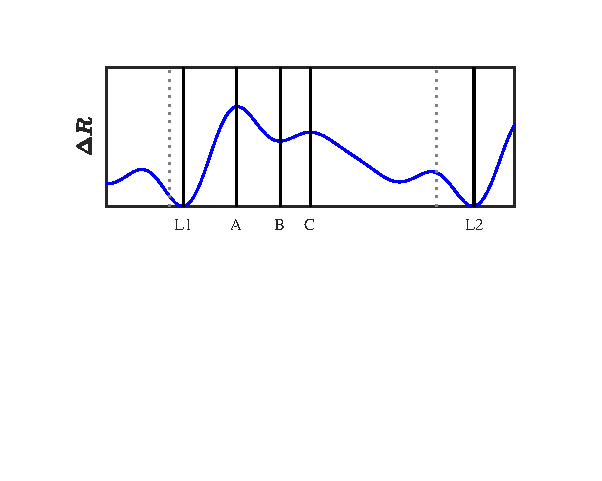
\includegraphics[width=0.9\textwidth,height=0.9\textheight,keepaspectratio]{figure5}    
	\caption{Normalise plot of impedance decrease during total occlusion.}
	\label{fig:normalise:total_occlusion}
\end{figure}
\mynote{Figure \ref{fig:normalise:venous_occlusion} is temporary. It needs to be improved by naming axis}

\begin{table}[h]
	\caption{Linear regression result for all participants during total occlusion.}
	\label{tbl:total_occlusion:region6}
	\centering
	\begin{tabu}{lcccccc}
		\toprule
		& \textbf{Slope [\si{\ohm/\second}]} & \textbf{Intercept [\si{\ohm}]} & \textbf{$R^2$} & \textbf{$Z_1$ [\si{\ohm}]} & \textbf{$Z_{end}$ [\si{\ohm}]} & \textbf{ $\Delta Z$ [\si{\ohm}]} \\ \midrule
	   	Participant 1  &  -0.00431  &  82.44   &      0.652 &   77.58 &  76.33  &   -1.25\\ 
		Participant 2  &   0.00044  &  96.55   &      0.105 &   97.22 &   97.28 &    0.07\\
		Participant 3  &  -0.00432  &  97.99   &      0.587 &   92.57 &   91.45 &   -1.12\\
		Participant 4  &   0.00226  &  60.31   &      0.789 &   63.31 &   63.45 &    0.14\\
		Participant 5  &  -0.00002  &  69.04   &     -0.005 &   69.22 &   69.01 &   -0.21\\
		Participant 6  &  -0.00096  &  58.38   &      0.457 &   57.34 &   56.95 &   -0.40\\
		Participant 7  &   0.00310  &  88.70   &      0.899 &   92.78 &   93.11 &    0.33\\
		Participant 8  &  -0.00080  &  79.94   &      0.644 &   78.97 &   78.82 &   -0.15\\ \bottomrule
	\end{tabu} 
\end{table}



%%********************************** % Section 5.3 ******************************************
\pagebreak
\section{Plethysmography impedance results}
\label{section5.3}
The iPG device provided a port illustrated as $Z_{AC}$ \mynote{To double check if this is the correct port name from the initial description} which provided a high-resolution view of the plethysmography waveform.  In fact, as shown in the design section xxx \mynote{Reference a section to this part}, the signal was amplified nearly 2500 times. Hence, the waveform obtained provides more detail and also improves rejection to noise.

The waveforms obtained through this method reproduce the change of volume per heart beat within the sensing electrodes. The filling of the blood vessels creates small changes in resistivity that change with the circulatory cycle (see section xxx \mynote{I have to add a section to describe how plethysmography is related to blood cycle}). The waveforms presented in this part were analysed using the decomposing method describe in section \ref{section4.3.2}. \mynote{I need to add more detail within that section}. Five different points on the waveform were identified by the algorithm.

The waveform produced by the device is inverted as represented by various other plethysmography devices such as photoplethysmography. During the systolic cycle, the blood vessels expand allowing more blood volume. Hence, the impedance drops proportionally to the amount of blood because the forearm's segment is more electrically conductive. On the other hand, during the diastolic cycle, blood vessels empty causing a reduction the quantity of blood contained in the segment. As a result, the impedance increases.  

Treating the digital signal required to remove noisy components of the waveform. As described in section xxx\mynote{Add section were the digital processing was performed}, the signal was levelled to zero.  From there, the points of interest were calculated to identify the different changes in the waveform. The analysis of the waveform was performed by averaging all the waveform detected by the algorithm. The following discussion represents the change of form from non-occlusion state to an occluded one. At the end of the section, the result of all participants will be summarised \mynote{I could add a description of how the signal looks. For instance by adding 10 or 20 beats to show how the device worked.}.

%%********************************** % Section 5.3.1 ******************************************
\subsection{Plethysmography waveform change from baseline to venous occlusion}
\label{section5.3.1}
This analysis corresponds to the waveform during baseline (\SIrange{0}{300}{\second}), venous occlusion (\SIrange{300}{480}{\second}) and return to control signal (\SIrange{480}{780}{\second}). This graph was obtained by averaging all the plethysmography waveforms detected by the algorithm and described in detail in section xxx \mynote{Add reference where the waveform detection algorithm is explained}. In the end, all the peaks were averaged obtaining the mean waveform displayed in the figure for baseline and venous occlusion.

Figure \ref{fig:iPG_venous_baseline} shows the common impedance plethysmography waveform, with indicators of their amplitudes at different points of interest. The distance between systolic peak (Point A) to dicrotic notch (Point B) and diastolic peak (Point C) was calculated. This value was later transposed into the occlusion wave to identify their values during the venous occlusion test.

As detailed in section xxx \mynote{Add note describing how the waveform is composed}, a plethysmography waveform consists of three distinct parts. The systolic peak, dicrotic notch and the diastolic peak, which have been indicated in the figure \ref{fig:iPG_venous_baseline}. From a qualitative point of view, it can be noticed that there is a difference in the morphology of the waveform. An analysis on the change of each these points are presented in figure \ref{fig:iPG_change_points_venous} and analysed in detail as follows.

\begin{figure*}[h]
	\centering
	\begin{subfigure}[t]{0.5\textwidth}
		\centering
		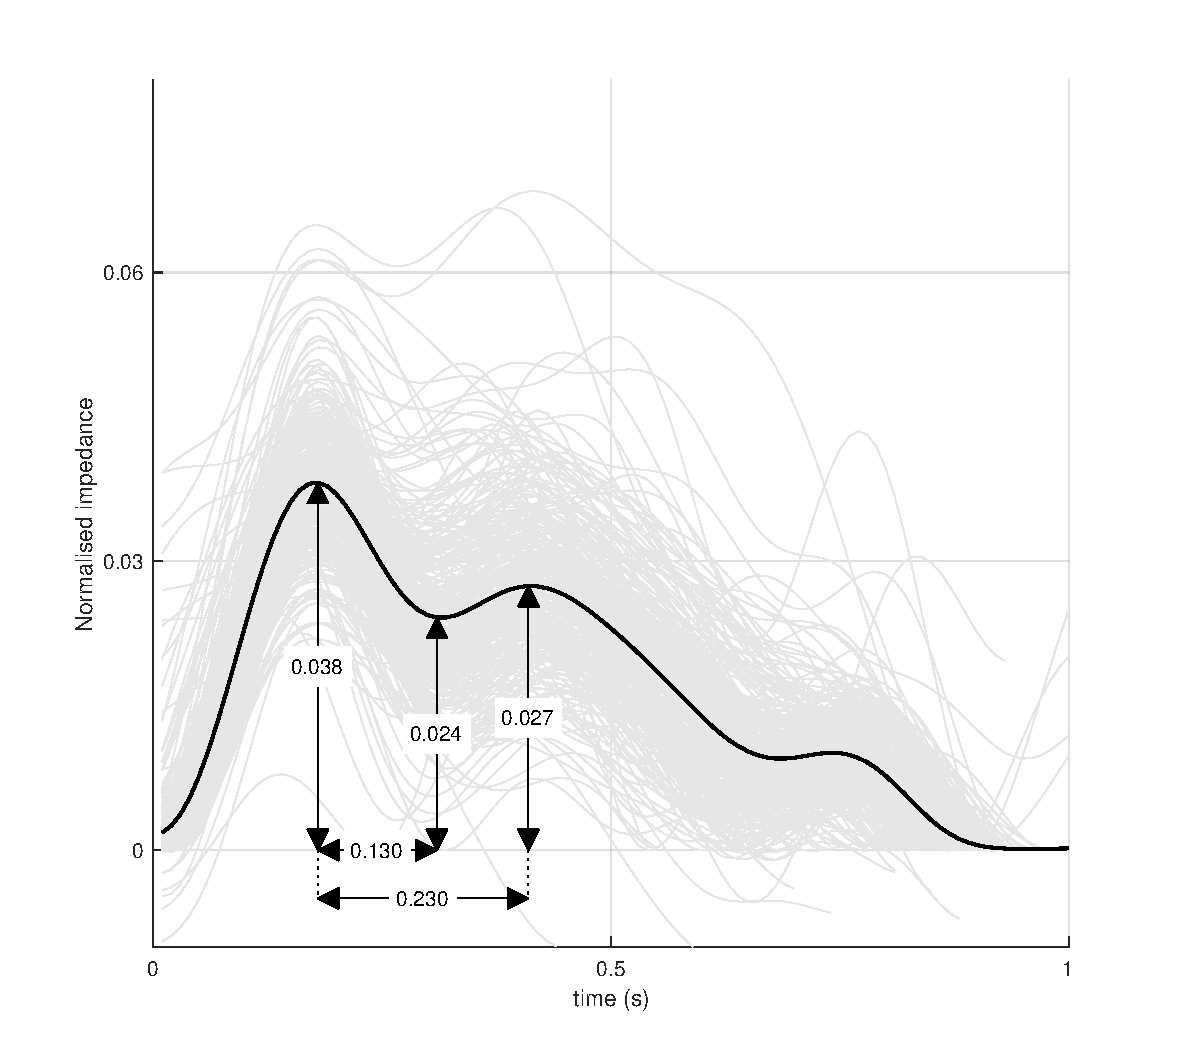
\includegraphics[height=7.6cm]{figure6a}
		\caption{Average plethysmography waveform for baseline region 1 (\SIrange{0}{300}{\second})}
		\label{fig:iPG_venous_baseline}
	\end{subfigure}%
	~ 
	\begin{subfigure}[t]{0.5\textwidth}
		\centering
		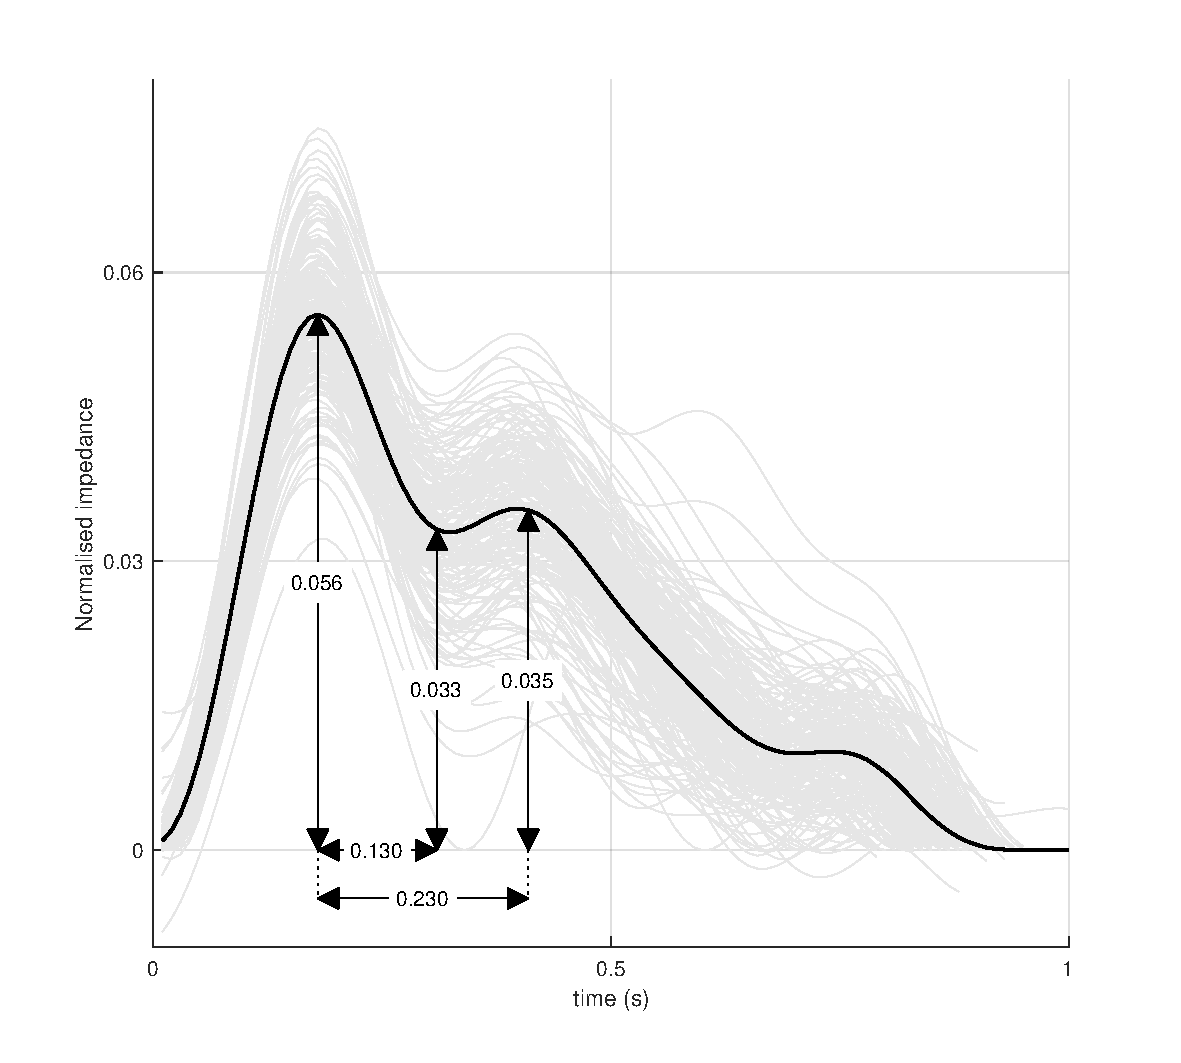
\includegraphics[height=7.6cm]{figure6b}
		\caption{Average plethysmography waveform during venous occlusion region 2 (\SIrange{300}{480}{\second})}
		\label{fig:iPG_venous_occlusion}
	\end{subfigure}
	\caption{Plethysmography waveform of the participant seven between baseline and venous occlusion}
	\label{fig:iPG_venous}
\end{figure*}

\begin{figure*}[h]
	\centering
	\begin{subfigure}[t]{0.5\textwidth}
	\centering
		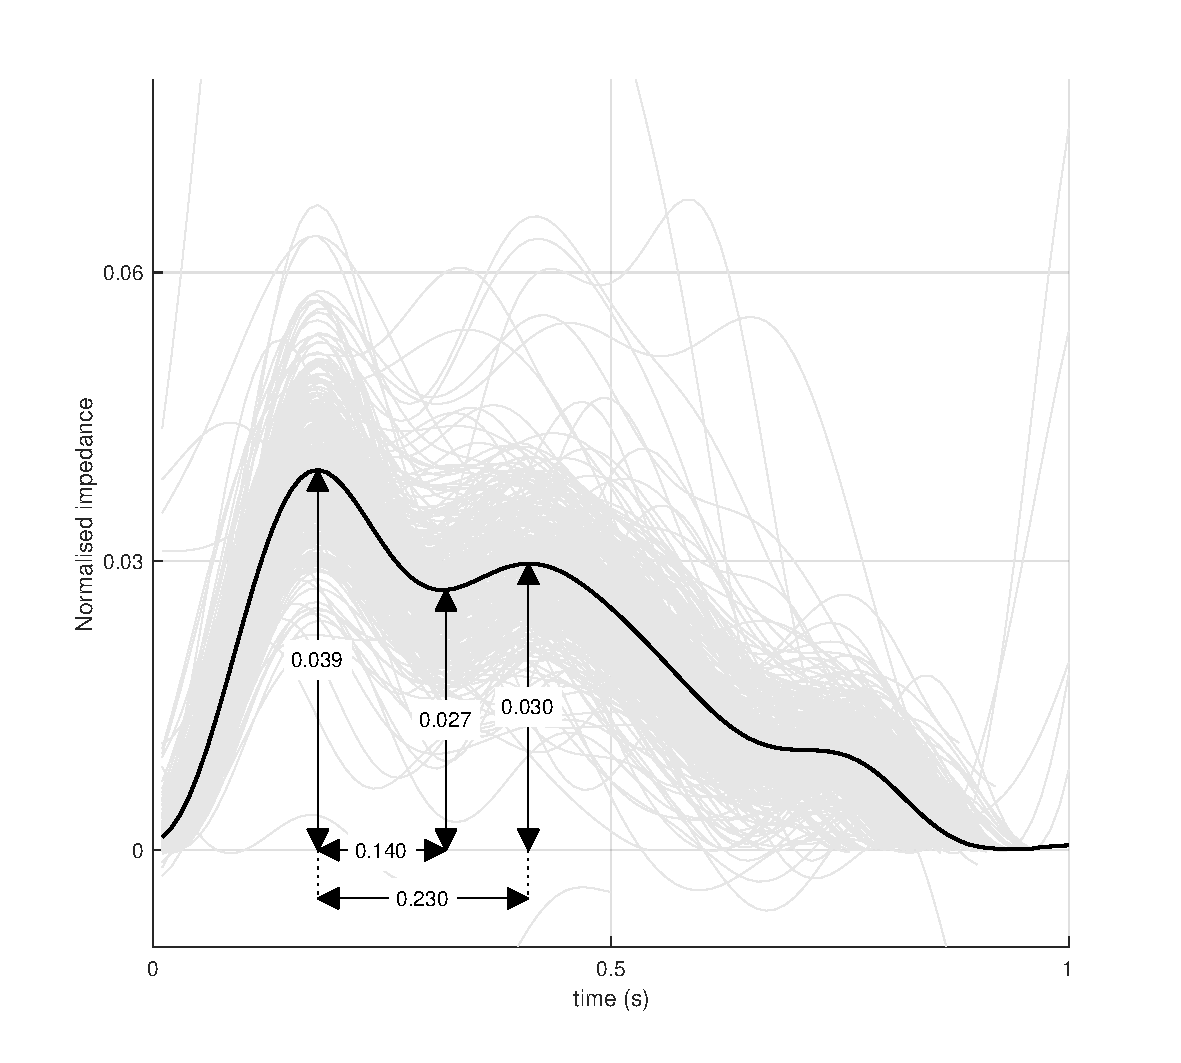
\includegraphics[height=6cm,keepaspectratio]{figure7a}    
		\caption{Change of amplitude of the waveform at point A.}
		\label{fig:change_A_venous}
	\end{subfigure}%
	~ 
	\begin{subfigure}[t]{0.5\textwidth}
		\centering
		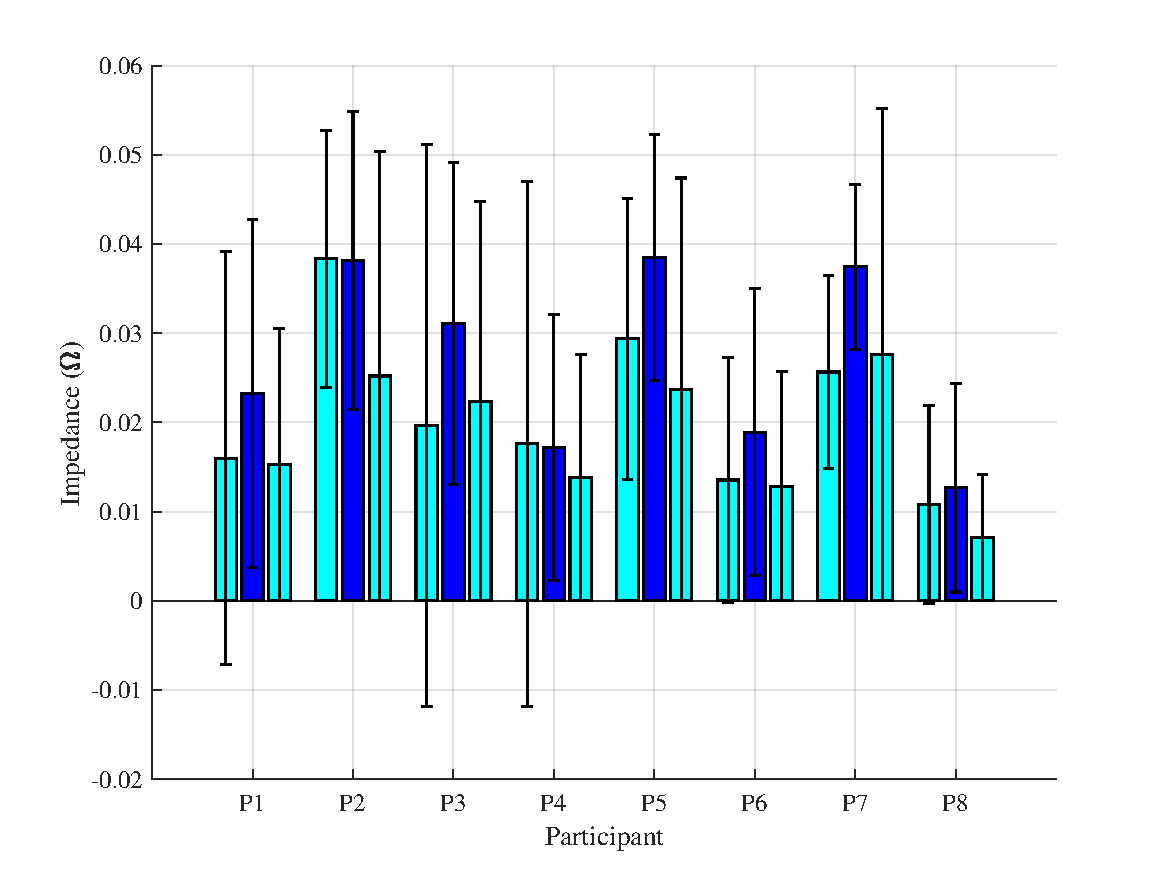
\includegraphics[height=6cm,keepaspectratio,keepaspectratio]{figure7b}    
		\caption{Change of amplitude of the waveform at point B}
		\label{fig:change_B_venous}
	\end{subfigure}
	~
	\begin{subfigure}[t]{0.5\textwidth}
		\centering
		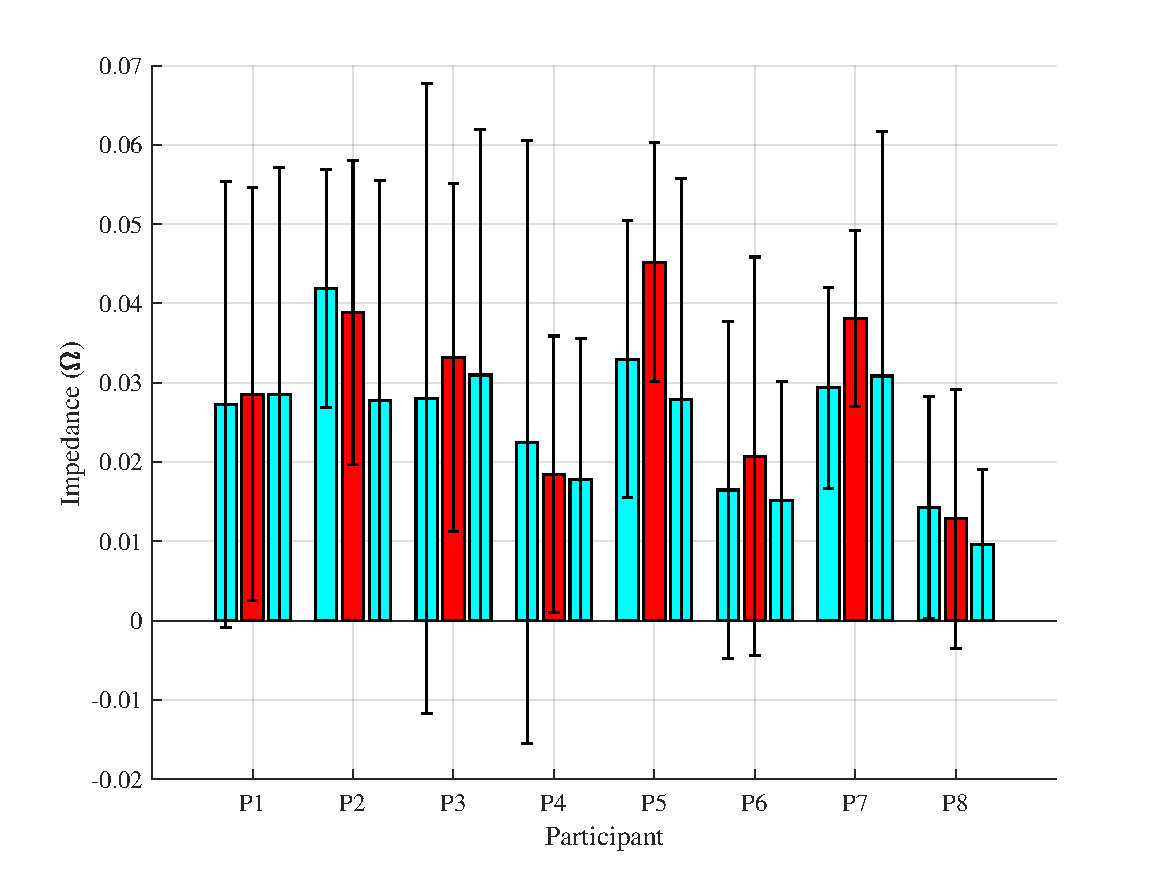
\includegraphics[height=6cm,keepaspectratio]{figure7c}    
		\caption{Change of amplitude of the waveform at point C}
		\label{fig:change_C_venous}
\end{subfigure}%
	\caption{Changes of the impedance peak values during baseline, partial arterial occlusion and return to baseline for points A,B and C.}
	\label{fig:iPG_change_points_venous}
\end{figure*}

\subsubsection{Changes in systolic peak (Point A)}
\label{section5.3.1.1}
Most of the signals showed a change on the height of their top systolic values after inflating the cuff to the values shown in column \textit{Occlusion 1} in Table~\ref{tbl:occlusions}. After quantifying the amplitude of the signal at this point, it can be seen an increase in their peak value. Indeed \SI{87}{\percent} of the participants showed an increment in resistance with an average of \SI{20.93}{\percent}, only participant 8 was an exception which impedance decreased \SI{-11.11}{\percent}. Then, when cuff's pressure was released, all the participants showed a decline of the peak value with an average of \SI{-27.88}{\percent}, returning to similar values previous the occlusion. Figure \ref{fig:change_A_venous} indicates the relation of change in amplitude during the three conditions. 

\begin{table}[h!]
	\caption{Change of amplitude of the waveform at peak A during the transition from baseline to venous occlusion.}
	\label{tbl:change_A_venous}
	\centering\small
\begin{tabular}{l
		*{3}{S[table-format=1.4]@{\,\( \pm \)\,}S[table-format=1.4]} %Format for Z+-std
		cc}
	\toprule
	& \multicolumn{2}{c}{\multirow{2}{*}{\textbf{Baseline [\si{\ohm}]}}}
	& \multicolumn{2}{c}{\multirow{2}{*}{\textbf{Occlusion [\si{\ohm}]}}}
	& \multicolumn{2}{c}{\multirow{2}{*}{\textbf{Baseline [\si{\ohm}]}}}
	& \multicolumn{2}{c}{\textbf{Change}} \\
	& \multicolumn{2}{c}{}
	& \multicolumn{2}{c}{}
	& \multicolumn{2}{c}{}
	&\textbf{R1-R2}&\textbf{R2-R3}\\\midrule
	Participant 1    &     0.0283    &     0.0233    &     0.0342    &     0.0191    &     0.0305    &     0.0305    &      20.93\%    &     -13.29\%    \\
	Participant 2    &     0.0491    &     0.0102    &     0.0595    &     0.0140    &     0.0449    &     0.0449    &      21.01\%    &     -29.68\%    \\
	Participant 3    &     0.0346    &     0.0351    &     0.0374    &     0.0144    &     0.0294    &     0.0294    &       7.91\%    &     -22.89\%    \\
	Participant 4    &     0.0252    &     0.0303    &     0.0272    &     0.0139    &     0.0222    &     0.0222    &       7.98\%    &     -19.87\%    \\
	Participant 5    &     0.0345    &     0.0112    &     0.0481    &     0.0098    &     0.0376    &     0.0376    &      39.68\%    &     -30.69\%    \\
	Participant 6    &     0.0233    &     0.0105    &     0.0306    &     0.0124    &     0.0251    &     0.0251    &      31.33\%    &     -23.52\%    \\
	Participant 7    &     0.0359    &     0.0080    &     0.0537    &     0.0081    &     0.0365    &     0.0365    &      49.72\%    &     -47.78\%    \\
	Participant 8    &     0.0237    &     0.0094    &     0.0211    &     0.0091    &     0.0127    &     0.0127    &     -11.11\%    &     -35.30\%    \\  \bottomrule
\end{tabular} 
\end{table}

\subsubsection{Changes in dicrotic notch peak (Point B)}
\label{section5.3.1.2}
The dicrotic notch point is located between the systolic and diastolic peaks. In the forearm's iPG waveform looks like a dip as illustrated figure \ref{fig:iPG_venous}. This locality in the waveform has been identified in this document as point B. 

The value of this signal changed from baseline when the venous occlusion happened. After that, when cuff was deflated, all impedance peaks decreased. According to the data shown on Table \ref{tbl:change_B_venous}, it can be noticed that most of the signals (\SI{75}{\percent}) shown an increase in their value. Certainly, there was an increment in impedance on average of \SI{29.30}{\percent}. However, partakers two and four noted a slight decrease in their values \SI{-0.47}{\percent} and \SI{-2.34}{\percent} which were not very significant compared to the others. In contrast, after releasing the pressure, all signals experience a reduction of their peak value (mean \SI{41.47}{\percent}).

\begin{table}[h!]
	\caption{Change of amplitude of the waveform at peak B during the transition from baseline to venous occlusion.}
	\label{tbl:change_B_venous}
	\centering\small
	\begin{tabular}{l
					*{3}{S[table-format=1.4]@{\,\( \pm \)\,}S[table-format=1.4]} %Format for Z+-std
					cc}
	\toprule
	& \multicolumn{2}{c}{\multirow{2}{*}{\textbf{Baseline [\si{\ohm}]}}}
	& \multicolumn{2}{c}{\multirow{2}{*}{\textbf{Occlusion [\si{\ohm}]}}}
	& \multicolumn{2}{c}{\multirow{2}{*}{\textbf{Baseline [\si{\ohm}]}}}
	& \multicolumn{2}{c}{\textbf{Change}} \\
	& \multicolumn{2}{c}{}
	& \multicolumn{2}{c}{}
	& \multicolumn{2}{c}{}
	&\textbf{R1-R2}&\textbf{R2-R3}\\\midrule
	Participant 1    &     0.0160    &     0.0231    &     0.0232    &     0.0195    &     0.0153    &     0.0153    &     45.07    \%      &     -49.54    \%      \\  
	Participant 2    &     0.0383    &     0.0144    &     0.0382    &     0.0167    &     0.0252    &     0.0252    &     -0.47    \%      &     -33.78    \%      \\  
	Participant 3    &     0.0196    &     0.0315    &     0.0311    &     0.0181    &     0.0224    &     0.0224    &     58.38    \%      &     -44.40    \%      \\  
	Participant 4    &     0.0176    &     0.0294    &     0.0172    &     0.0149    &     0.0138    &     0.0138    &     -2.34    \%      &     -19.25    \%      \\  
	Participant 5    &     0.0294    &     0.0158    &     0.0385    &     0.0138    &     0.0237    &     0.0237    &     31.07    \%      &     -50.37    \%      \\  
	Participant 6    &     0.0135    &     0.0138    &     0.0189    &     0.0161    &     0.0128    &     0.0128    &     39.49    \%      &     -44.62    \%      \\  
	Participant 7    &     0.0256    &     0.0108    &     0.0374    &     0.0092    &     0.0276    &     0.0276    &     45.94    \%      &     -38.44    \%      \\  
	Participant 8    &     0.0108    &     0.0111    &     0.0127    &     0.0117    &     0.0071    &     0.0071    &     17.28    \%      &     -51.42    \%      \\ \bottomrule
	\end{tabular} 
\end{table}

\subsubsection{Changes in diastolic peak (Point C)}
\label{section5.3.1.3}
The diastolic peak corresponds to the point C of the waveform. Figure \ref{fig:change_C_venous} shows that there is not a clear trend compared to the other spots previously examined. In fact, three participants experience a decline in the impedance at this point with an average drop of \SI{-11.74}{\percent} and the rest experienced an increase of impedance had a rise an average of \SI{23}{\percent}. Table \ref{tbl:change_C_venous} shows the mean values of the impedance at this place. At this point, it is not possible to get a conclusion about the trend of this point of data. In contrast, after releasing the upper arm's pressure, most participants experience a decrease in their diastolic peak impedance, with an average of \SI{-24}{\percent}. Participant one was the only one that did not register any significant change. 

\begin{table}[h!]
	\caption{Change of amplitude of the waveform at peak C during the transition from baseline to venous occlusion.}
	\label{tbl:change_C_venous}
	\centering\small
	\begin{tabular}{l
					*{3}{S[table-format=1.4]@{\,\( \pm \)\,}S[table-format=1.4]} %Format for Z+-std
					cc}
	\toprule
	& \multicolumn{2}{c}{\multirow{2}{*}{\textbf{Baseline [\si{\ohm}]}}}
	& \multicolumn{2}{c}{\multirow{2}{*}{\textbf{Occlusion [\si{\ohm}]}}}
	& \multicolumn{2}{c}{\multirow{2}{*}{\textbf{Baseline [\si{\ohm}]}}}
	& \multicolumn{2}{c}{\textbf{Change}} \\
	& \multicolumn{2}{c}{}
	& \multicolumn{2}{c}{}
	& \multicolumn{2}{c}{}
	&\textbf{R1-R2}&\textbf{R2-R3}\\\midrule
	Participant 1    &     0.0272    &     0.0281    &     0.0285    &     0.0260    &     0.0286    &     0.0286    &       4.79    \%      &       0.03    \%      \\  
	Participant 2    &     0.0419    &     0.0150    &     0.0389    &     0.0191    &     0.0278    &     0.0278    &      -7.17    \%      &     -26.57    \%      \\  
	Participant 3    &     0.0280    &     0.0397    &     0.0332    &     0.0219    &     0.0310    &     0.0310    &      18.37    \%      &      -7.80    \%      \\  
	Participant 4    &     0.0225    &     0.0380    &     0.0185    &     0.0174    &     0.0178    &     0.0178    &     -17.99    \%      &      -2.94    \%      \\  
	Participant 5    &     0.0330    &     0.0175    &     0.0452    &     0.0151    &     0.0279    &     0.0279    &      37.18    \%      &     -52.58    \%      \\  
	Participant 6    &     0.0165    &     0.0212    &     0.0207    &     0.0251    &     0.0151    &     0.0151    &      25.96    \%      &     -34.25    \%      \\  
	Participant 7    &     0.0294    &     0.0127    &     0.0381    &     0.0111    &     0.0309    &     0.0309    &      29.85    \%      &     -24.77    \%      \\  
	Participant 8    &     0.0143    &     0.0140    &     0.0129    &     0.0163    &     0.0096    &     0.0096    &     -10.06    \%      &     -23.09    \%      \\  
	\bottomrule
	\end{tabular} 
\end{table}

%%********************************** % Section 5.3.2 ******************************************
\subsection{Plethysmography waveform change during partial arterial occlusion}
\label{section5.3.2}
During this type of occlusion, most of the signals also showed a modification on the height of their top systolic values. The analysis of this section resembles the baseline time in region 3 (\SIrange{480}{780}{\second}), three minutes of partial venous occlusion in region 4 (\SIrange{780}{960}{\second}) and return to baseline region 5 (\SIrange{960}{1260}{\second}). The cuff was inflated to the pressure presented in the column \textit{Occlusion 2} in Table \ref{tbl:occlusions}. 

Figure \ref{fig:iPG_change_points_arterial} shows the average waveform in baseline and during occlusion for participant seven. As it can be seen from the graph, it is apparent that there is an increase in the systolic peak (point A) and a reduction in the diastolic peak point C). Figure \ref{fig:iPG_change_points_arterial} also features the impedance change in each participant. The following sections will describe in detail the changes to each of the spots. 

\begin{figure*}[t!]
	\centering
	\begin{subfigure}[t]{0.5\textwidth}
		\centering
		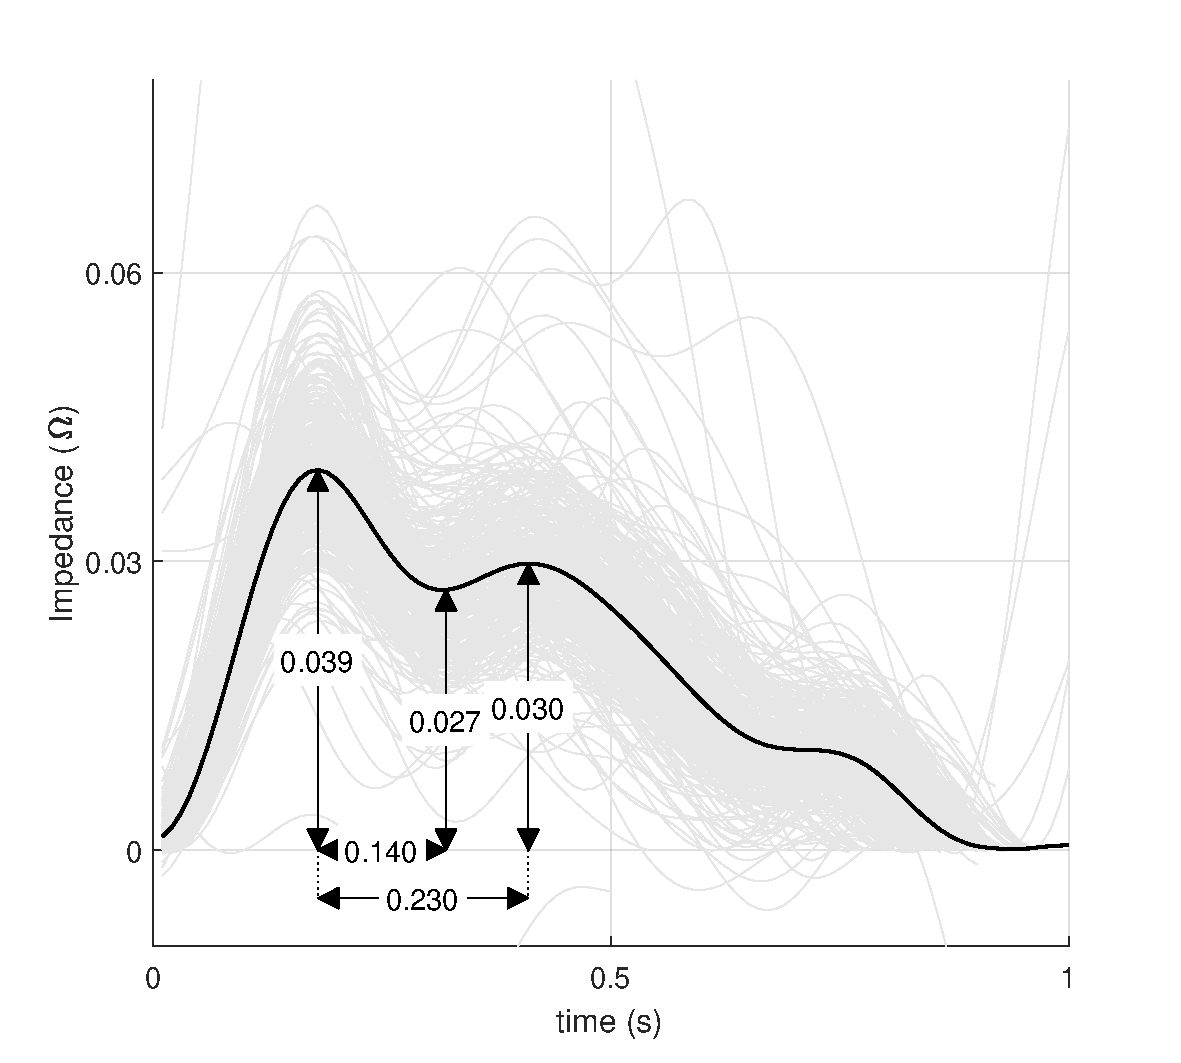
\includegraphics[height=7.6cm]{figure8a}
		\caption{Average plethysmography waveform during venous occlusion region 3 (\SIrange{480}{780}{\second})}
		\label{fig:iPG_arterial_baseline}
	\end{subfigure}%
	~ 
	\begin{subfigure}[t]{0.5\textwidth}
		\centering
		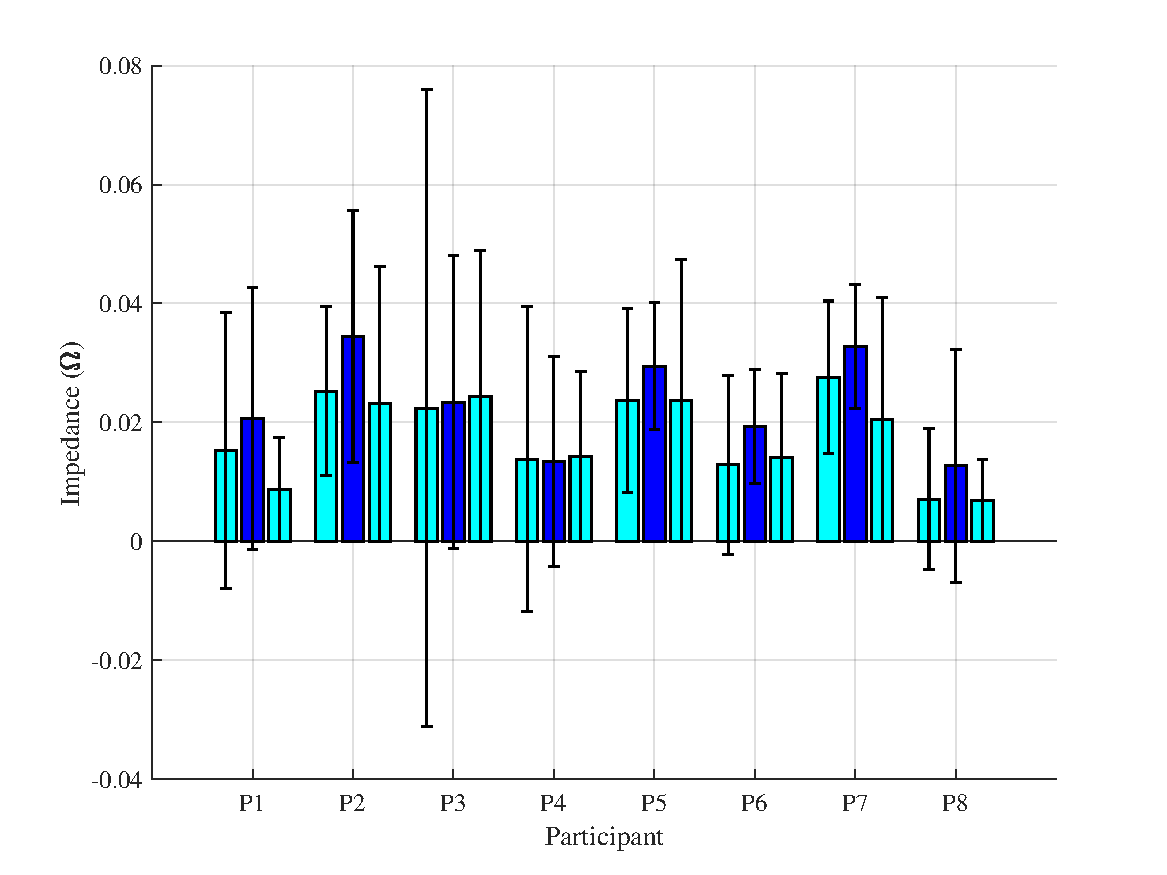
\includegraphics[height=7.6cm]{figure8b}
		\caption{Average plethysmography waveform during venous occlusion region 4 (\SIrange{780}{960}{\second})}
		\label{fig:iPG_arterial_occlusion}
	\end{subfigure}
	\caption{Plethysmography waveform of the participant seven between baseline and partial arterial occlusion}
	\label{fig:iPG_arterial}
\end{figure*}

\begin{figure*}[t!]
	\centering
	\begin{subfigure}[t]{0.5\textwidth}
		\centering
		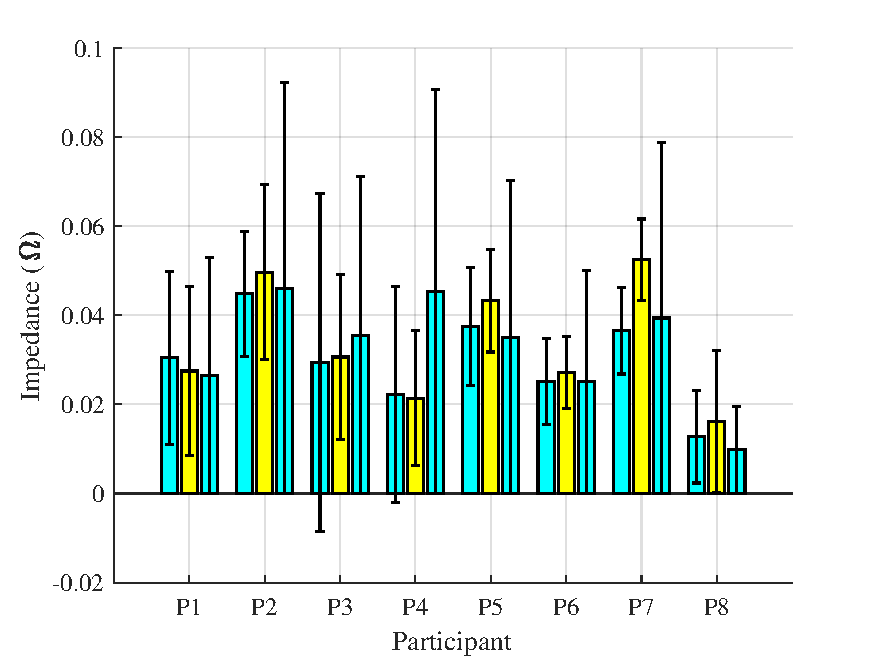
\includegraphics[height=6cm,keepaspectratio]{figure9a}    
		\caption{Change of amplitude of the waveform at point A.}
		\label{fig:change_A_arterial}
	\end{subfigure}%
	~ 
	\begin{subfigure}[t]{0.5\textwidth}
		\centering
		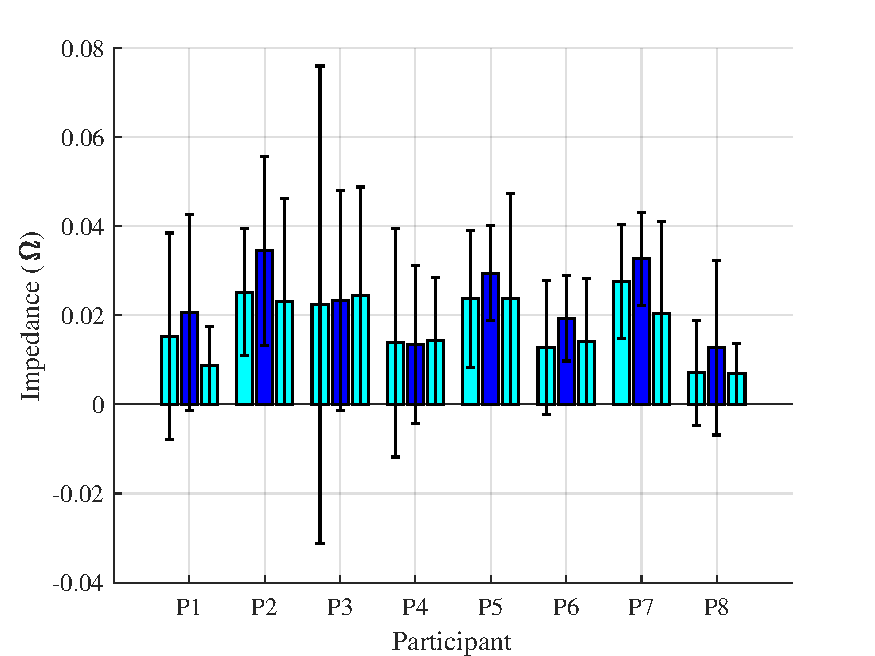
\includegraphics[height=6cm,keepaspectratio,keepaspectratio]{figure9b}    
		\caption{Change of amplitude of the waveform at point B}
		\label{fig:change_B_arterial}
	\end{subfigure}
	~
	\begin{subfigure}[t]{0.5\textwidth}
		\centering
		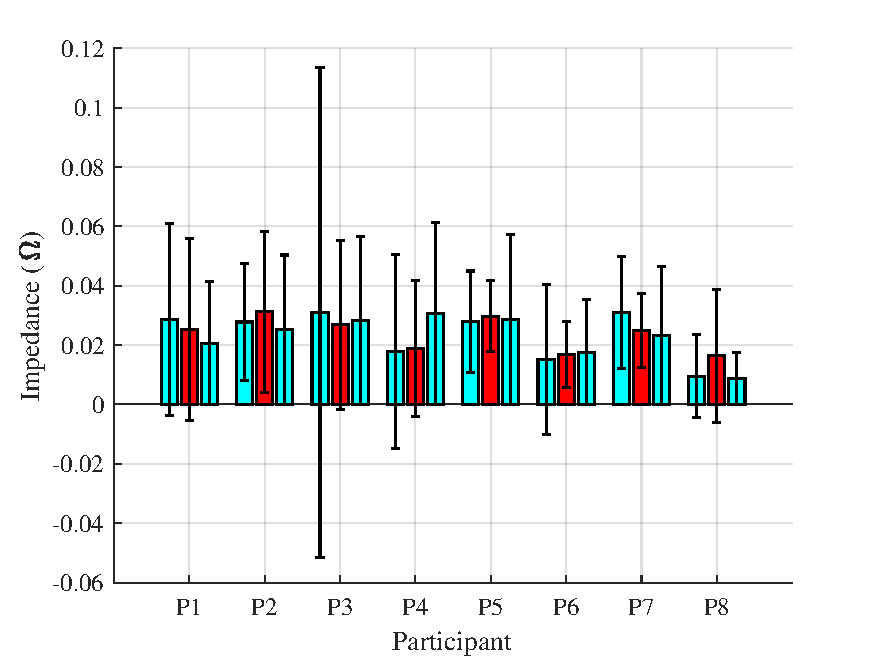
\includegraphics[height=6cm,keepaspectratio]{figure9c}    
		\caption{Change of amplitude of the waveform at point C}
		\label{fig:change_C_arterial}
	\end{subfigure}%
	\caption{Changes of the impedance peak values during baseline, partial arterial occlusion and return to baseline for points A,B and C.}
	\label{fig:iPG_change_points_arterial}
\end{figure*}

\subsubsection{Changes in systolic peak (Point A)}
\label{section5.3.2.1}
Through this occlusive event, six participants (\SI{75}{\percent}) experienced an increase in electrical resistivity in the point A. The average increase was about \SI{18.10}{\percent}.  On the other hand, the participants whose impedance decreased was in average \ SI {-6.77} {\ percent}. In general, it can be noticed the growth at this point. Figure \ref{fig:change_A_arterial} shows the change in amplitude for each one. Table \ref{tbl:change_A_arterial} summarises the average impedances and the changes in each region. 

After the cuff was deflated, the peak impedance of most of the participants (\SI{75}{\percent})  decreased in mean \SI{-21.13}{\percent}).  In contrast, participants three and four showed an increase in impedance of \SI{12.71}{\percent} and \SI{107.91}{\percent}. A large number of the latter being compared to its standard deviation shows that there must be noise in the signal affecting its quality.   

\begin{table}[h!]
	\caption{Change of amplitude of the waveform at peak A during the transition from baseline to venous occlusion.}
	\label{tbl:change_A_arterial}
	\centering\small
	\begin{tabular}{l
			*{3}{S[table-format=1.4]@{\,\( \pm \)\,}S[table-format=1.4]} %Format for Z+-std
			cc}
		\toprule
		& \multicolumn{2}{c}{\multirow{2}{*}{\textbf{Baseline [\si{\ohm}]}}}
		& \multicolumn{2}{c}{\multirow{2}{*}{\textbf{Occlusion [\si{\ohm}]}}}
		& \multicolumn{2}{c}{\multirow{2}{*}{\textbf{Baseline [\si{\ohm}]}}}
		& \multicolumn{2}{c}{\textbf{Change}} \\
		& \multicolumn{2}{c}{}
		& \multicolumn{2}{c}{}
		& \multicolumn{2}{c}{}
		&\textbf{R1-R2}&\textbf{R2-R3}\\\midrule
		Participant 1    &     0.0305    &     0.0194    &     0.0275    &     0.0190    &     0.0265    &     0.0265    &     -9.73    \%      &      -3.30    \%      \\  
		Participant 2    &     0.0449    &     0.0140    &     0.0497    &     0.0197    &     0.0461    &     0.0461    &     10.74    \%      &      -8.02    \%      \\  
		Participant 3    &     0.0294    &     0.0379    &     0.0307    &     0.0185    &     0.0356    &     0.0356    &      4.11    \%      &      16.71    \%      \\  
		Participant 4    &     0.0222    &     0.0242    &     0.0214    &     0.0152    &     0.0453    &     0.0453    &     -3.81    \%      &     107.91    \%      \\  
		Participant 5    &     0.0376    &     0.0133    &     0.0433    &     0.0115    &     0.0351    &     0.0351    &     15.30    \%      &     -21.83    \%      \\  
		Participant 6    &     0.0251    &     0.0096    &     0.0272    &     0.0081    &     0.0251    &     0.0251    &      8.30    \%      &      -8.36    \%      \\  
		Participant 7    &     0.0365    &     0.0097    &     0.0525    &     0.0092    &     0.0394    &     0.0394    &     43.53    \%      &     -35.69    \%      \\  
		Participant 8    &     0.0127    &     0.0104    &     0.0161    &     0.0160    &     0.0098    &     0.0098    &     26.65    \%      &     -49.61    \%      \\      
		\bottomrule
	\end{tabular} 
\end{table}

\subsubsection{Changes in dicrotic notch peak (Point B)}
\label{section5.3.2.2}
In the dicrotic notch position (point B), there was a similar trend as the one seen in the systolic peak. In total, seven out of eight participants registered an increase of impedance. The average increase at the dicrotic notch was about \SI{35.52}{\percent}. Only participant four showed a  slight drop in impedance (\SI{-2.44}{\percent}).  

When the pressure was removed, six out of eight of the study members experience a fall in electrical resistivity. In averaged, it reduced \SI{-52.39}{\percent}. Again, participant four was the exception to this reduction, as well as participant three. Their impedance rose \SI{5.72}{\percent} and \SI{4.61}{\percent}.

Figure \ref{fig:change_B_arterial} evidences these changes in each region. Table \ref{fig:change_B_arterial} details the mean impedances and the ratio of change between each region.

\begin{table}[h!]
	\caption{Change of amplitude of the waveform at peak B during the transition from baseline to venous occlusion.}
	\label{tbl:change_B_arterial}
	\centering\small
	\begin{tabular}{l
			*{3}{S[table-format=1.4]@{\,\( \pm \)\,}S[table-format=1.4]} %Format for Z+-std
			cc}
		\toprule
		& \multicolumn{2}{c}{\multirow{2}{*}{\textbf{Baseline [\si{\ohm}]}}}
		& \multicolumn{2}{c}{\multirow{2}{*}{\textbf{Occlusion [\si{\ohm}]}}}
		& \multicolumn{2}{c}{\multirow{2}{*}{\textbf{Baseline [\si{\ohm}]}}}
		& \multicolumn{2}{c}{\textbf{Change}} \\
		& \multicolumn{2}{c}{}
		& \multicolumn{2}{c}{}
		& \multicolumn{2}{c}{}
		&\textbf{R1-R2}&\textbf{R2-R3}\\\midrule
		Participant 1    &     0.0153    &     0.0232    &     0.0206    &     0.0220    &     0.0087    &     0.0087    &     35.05    \%      &     -77.89    \%      \\  
		Participant 2    &     0.0252    &     0.0142    &     0.0345    &     0.0212    &     0.0231    &     0.0231    &     36.75    \%      &     -44.93    \%      \\  
		Participant 3    &     0.0224    &     0.0536    &     0.0234    &     0.0247    &     0.0244    &     0.0244    &      4.42    \%      &       4.61    \%      \\  
		Participant 4    &     0.0138    &     0.0256    &     0.0135    &     0.0177    &     0.0143    &     0.0143    &     -2.44    \%      &       5.72    \%      \\  
		Participant 5    &     0.0237    &     0.0155    &     0.0294    &     0.0107    &     0.0237    &     0.0237    &     24.19    \%      &     -24.13    \%      \\  
		Participant 6    &     0.0128    &     0.0150    &     0.0193    &     0.0096    &     0.0141    &     0.0141    &     50.42    \%      &     -40.66    \%      \\  
		Participant 7    &     0.0276    &     0.0128    &     0.0327    &     0.0104    &     0.0205    &     0.0205    &     18.66    \%      &     -44.28    \%      \\  
		Participant 8    &     0.0071    &     0.0118    &     0.0127    &     0.0196    &     0.0069    &     0.0069    &     79.15    \%      &     -82.44    \%      \\    
\bottomrule
	\end{tabular} 
\end{table}

\subsubsection{Changes in diastolic peak (Point C)}
\label{section5.3.2.3}
Changes in the diastolic peak also presented a similar trend as seen in points A and B. However; the changes were not as marked as the ones seen before. Figure \ref{fig:change_C_arterial} and Table \ref{tbl:change_C_arterial} summarise the values obtained. In total, \SI{62.5}{\percent} showed an increase of impedance between region 3 and 4. It increased with a median of \SI{21.68}{\percent}. Participant eight showed a change significantly larger than the mean (\SI{71.41}{\percent}). Others study members pointed a decrease of electrical resistivity in \SI{-14.71}{\percent} in average.  

On the opposite side of the exercise, after releasing the pressure, a similar number of partakers whose peak increased showed a reduction in impedance (\SI{62.5}{\percent}).  However, these were different members. In average, impedance reduced \SI{-25.56}{\percent} in total. Again, participant eight showed a greater ratio of change significantly exceeding the mean. On the other hand, participants that exhibited an increase of impedance, the average was \SI{25.23}{\percent}. Participant four outperformed notably the average ratio (\SI{66.03}{\percent}).

\begin{table}[h!]
	\caption{Change of amplitude of the waveform at peak C during the transition from baseline to venous occlusion.}
	\label{tbl:change_C_arterial}
	\centering\small
	\begin{tabular}{l
			*{3}{S[table-format=1.4]@{\,\( \pm \)\,}S[table-format=1.4]} %Format for Z+-std
			cc}
		\toprule
		& \multicolumn{2}{c}{\multirow{2}{*}{\textbf{Baseline [\si{\ohm}]}}}
		& \multicolumn{2}{c}{\multirow{2}{*}{\textbf{Occlusion [\si{\ohm}]}}}
		& \multicolumn{2}{c}{\multirow{2}{*}{\textbf{Baseline [\si{\ohm}]}}}
		& \multicolumn{2}{c}{\textbf{Change}} \\
		& \multicolumn{2}{c}{}
		& \multicolumn{2}{c}{}
		& \multicolumn{2}{c}{}
		&\textbf{R1-R2}&\textbf{R2-R3}\\\midrule
		Participant 1    &     0.0286    &     0.0323    &     0.0253    &     0.0307    &     0.0206    &     0.0206    &     -11.44    \%      &     -16.31    \%      \\  
		Participant 2    &     0.0278    &     0.0196    &     0.0312    &     0.0272    &     0.0252    &     0.0252    &      12.45    \%      &     -21.78    \%      \\  
		Participant 3    &     0.0310    &     0.0826    &     0.0268    &     0.0284    &     0.0283    &     0.0283    &     -13.49    \%      &       4.71    \%      \\  
		Participant 4    &     0.0178    &     0.0327    &     0.0189    &     0.0229    &     0.0306    &     0.0306    &       5.94    \%      &      66.03    \%      \\  
		Participant 5    &     0.0279    &     0.0171    &     0.0298    &     0.0119    &     0.0287    &     0.0287    &       6.74    \%      &      -3.96    \%      \\  
		Participant 6    &     0.0151    &     0.0252    &     0.0169    &     0.0111    &     0.0176    &     0.0176    &      11.86    \%      &       4.96    \%      \\  
		Participant 7    &     0.0309    &     0.0189    &     0.0249    &     0.0124    &     0.0232    &     0.0232    &     -19.19    \%      &      -5.65    \%      \\  
		Participant 8    &     0.0096    &     0.0139    &     0.0164    &     0.0224    &     0.0087    &     0.0087    &      71.41    \%      &     -80.09    \%      \\  

		\bottomrule
	\end{tabular} 
\end{table}

\subsection{Plethysmography waveform change during total occlusion}
\label{section5.3.3}
Performing total occlusion completely blocks the inflow and outflow of blood beneath the arm's cuff.  Hence, there is no change of volume within the arm's segment. As a result, impedance plethysmography should not present changes.  Figure \ref{fig:iPG_total} shows the plethysmography baseline in region 5 (\SIrange{960}{1260}{\second}) and region 6  (\SIrange{1260}{1440}{\second}) of participant seven. As portrayed by the Figure \ref{fig:iPG_change_points_total}, the amplitudes of most of the participants dropped during the occlusion.

However, participant four experience different behaviour in all the points. The standard deviation of this participant also suggests that there would have been a problem with his plethysmography signal during the test. 

In general, point A decreased in average \SI{-66.15}{\percent} its peak value occlusion. Then when the pressure was released, impedance recovered its value in \SI{75.98}{\percent}. A similar event occurred with point B; peak signals dropped a median of \SI{-63.29}{\percent} during blockage and recovered in average to \SI{74.02}{\percent}. Alike, point C, decreased in average \SI{-50.27}{\percent}  and increased \SI{58.71}{\percent} after the occlusion.

\begin{figure*}[t!]
	\centering
	\begin{subfigure}[t]{0.5\textwidth}
		\centering
		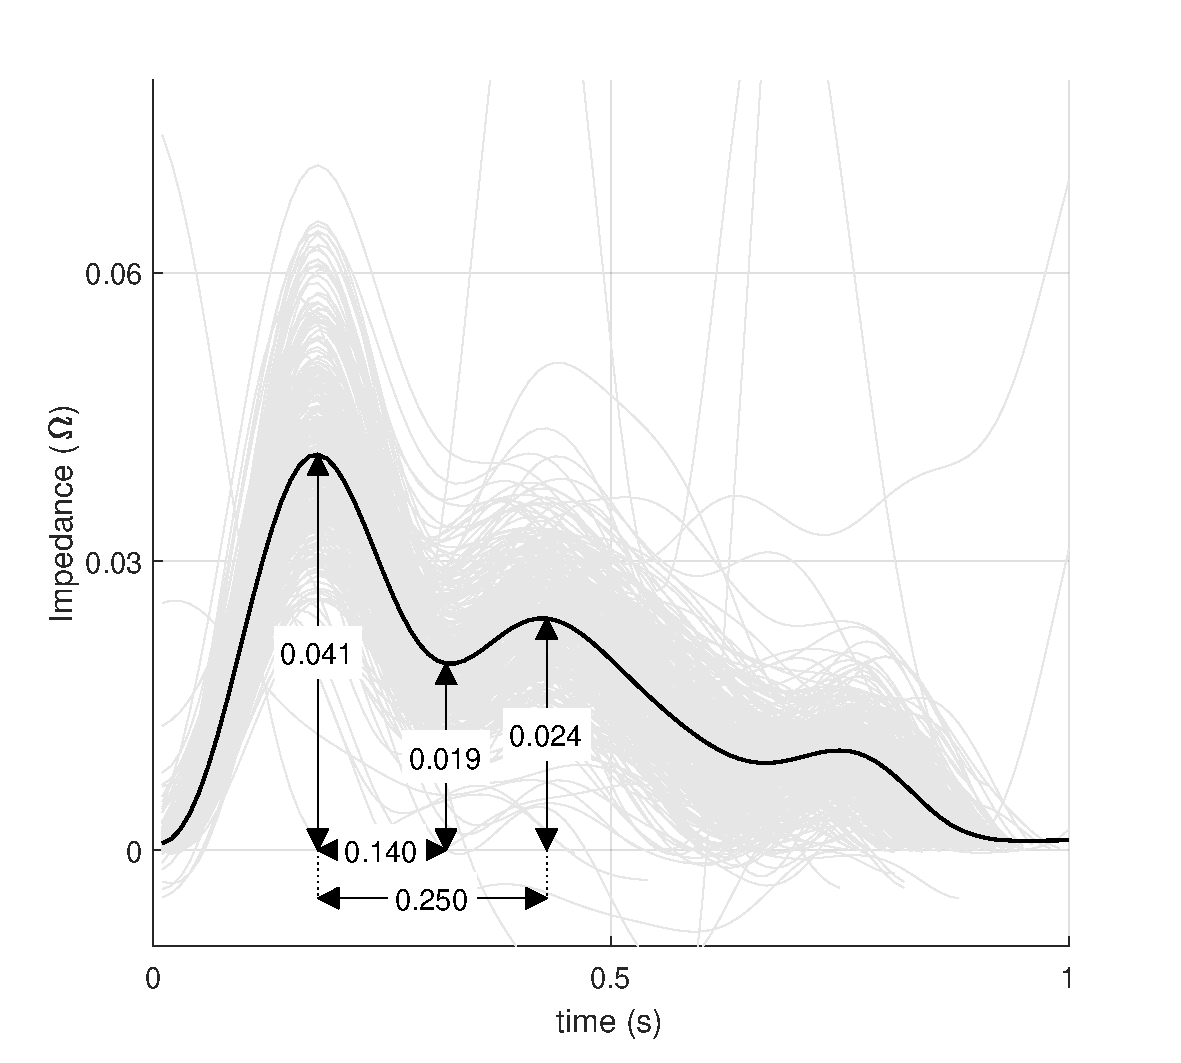
\includegraphics[height=7.6cm]{figure10a}
		\caption{Average plethysmography waveform during venous occlusion region 5 (\SIrange{960}{1260}{\second})}
		\label{fig:iPG_total_baseline}
	\end{subfigure}%
	~ 
	\begin{subfigure}[t]{0.5\textwidth}
		\centering
		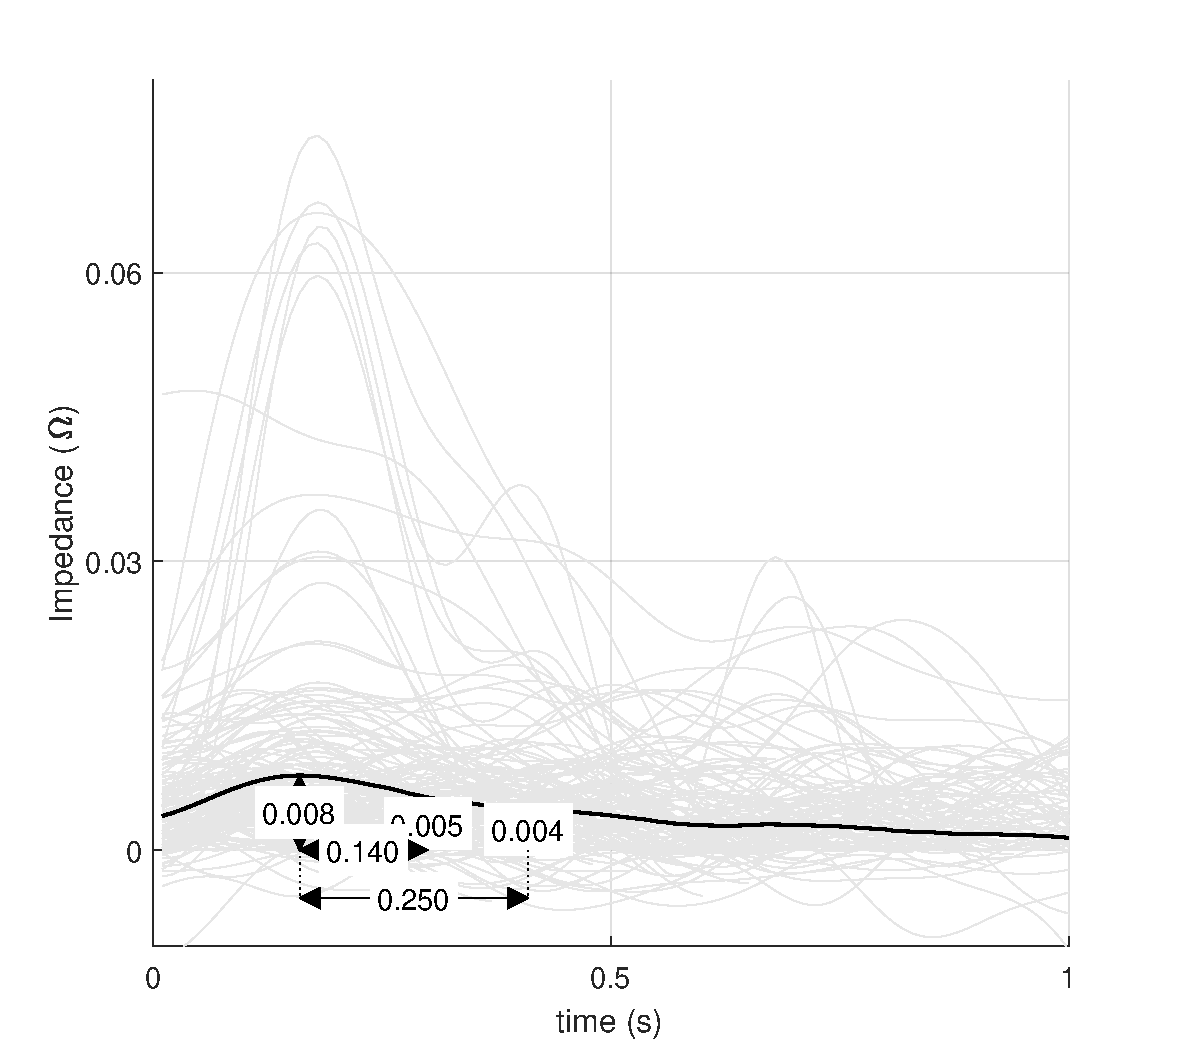
\includegraphics[height=7.6cm]{figure10b}
		\caption{Average plethysmography waveform during venous occlusion region 6 (\SIrange{1260}{1440}{\second})}
		\label{fig:iPG_total_occlusion}
	\end{subfigure}
	\caption{Plethysmography waveform of the participant seven between baseline and total occlusion}
	\label{fig:iPG_total}
\end{figure*}

\begin{figure*}[t!]
	\centering
	\begin{subfigure}[t]{0.5\textwidth}
		\centering
		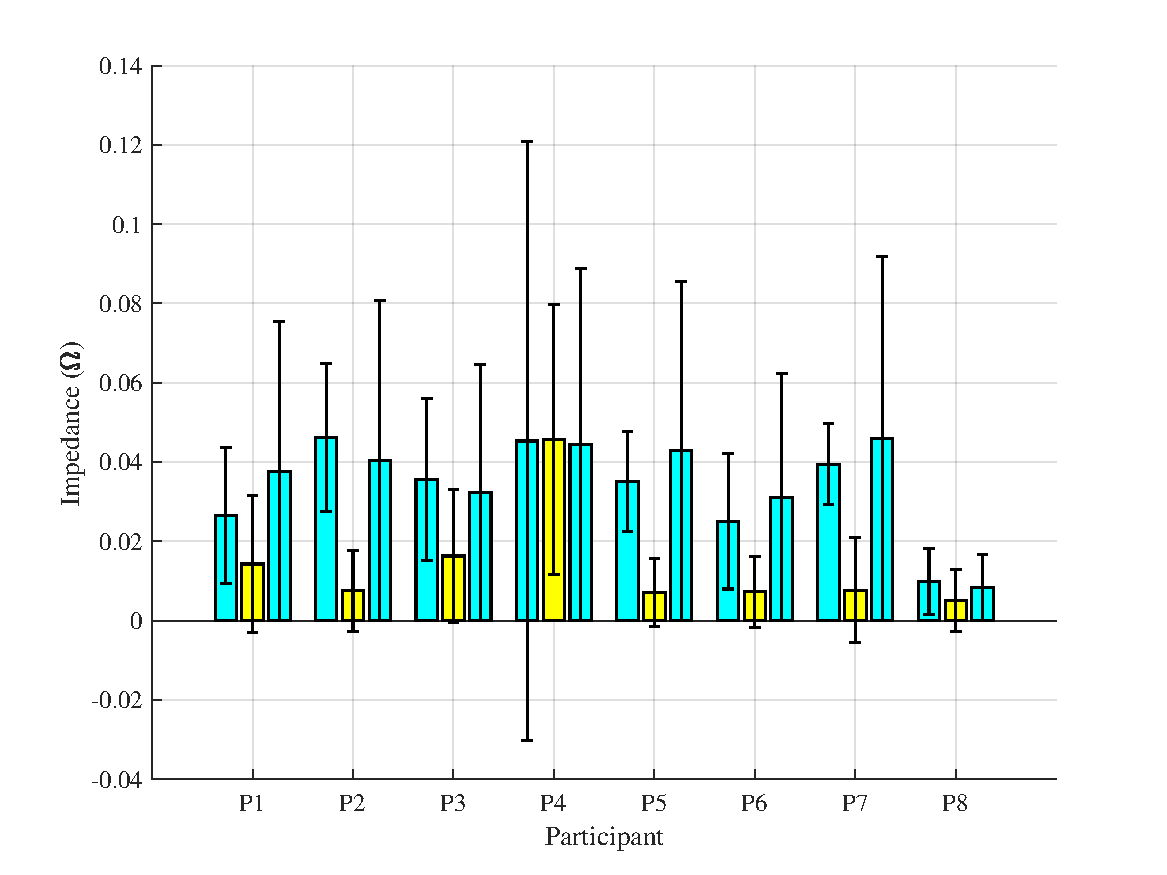
\includegraphics[height=6cm,keepaspectratio]{figure11a}    
		\caption{Change of amplitude of the waveform at point A.}
		\label{fig:change_A_total}
	\end{subfigure}%
	~ 
	\begin{subfigure}[t]{0.5\textwidth}
		\centering
		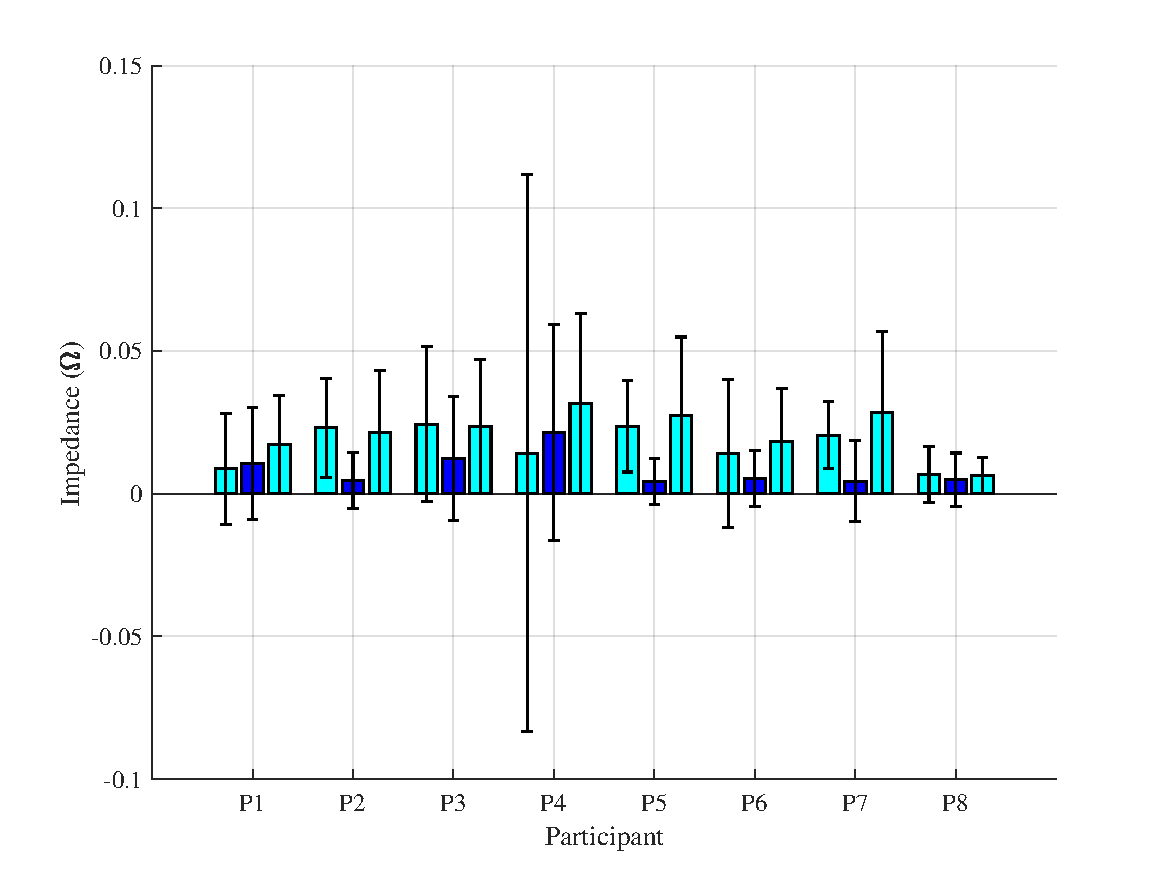
\includegraphics[height=6cm,keepaspectratio,keepaspectratio]{figure11b}    
		\caption{Change of amplitude of the waveform at point B}
		\label{fig:change_B_total}
	\end{subfigure}
	~
	\begin{subfigure}[t]{0.5\textwidth}
		\centering
		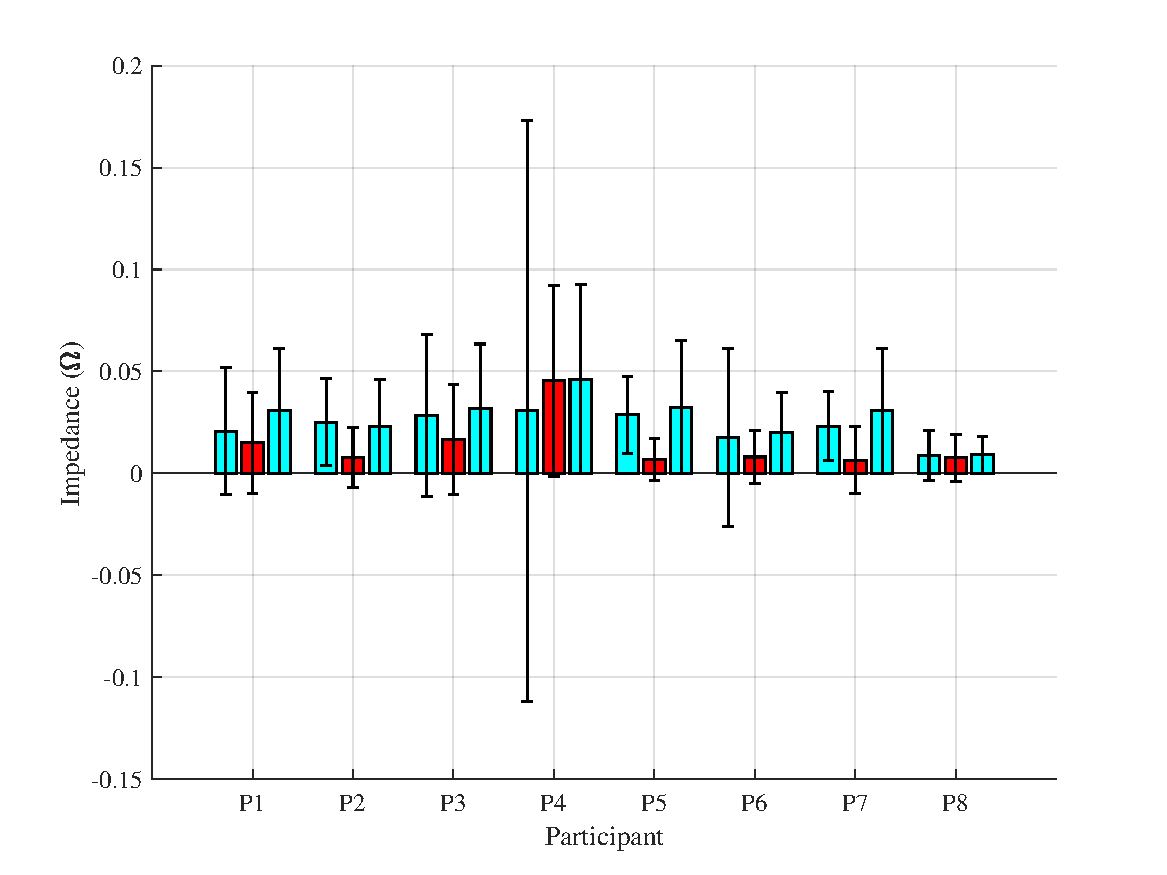
\includegraphics[height=6cm,keepaspectratio]{figure11c}    
		\caption{Change of amplitude of the waveform at point C}
		\label{fig:change_C_total}
	\end{subfigure}%
	\caption{Changes of the impedance peak values during baseline, total occlusion and return to baseline for points A,B and C.}
	\label{fig:iPG_change_points_total}
\end{figure*}


%%********************************** % Section 5.4 ******************************************
\pagebreak
\section{Blood flow calculation from baseline signal}
\label{section5.4}

%********************************** % Section 5.4.1 ******************************************
\subsection{Blood flow calculation using venous occlusion plethysmography}
\label{section5.4.1}
Using the method venous occlusion plethysmography is possible to calculate the blood flow in the forearm segment. As it can be seen from figure \ref{fig:blood_flow:venous_occlusion} the data is not dropping in a completely straight line. As a reminder, the occlusion occurred during \SIrange{300}{480}{\second} which is the time lapse showed. There are impedance variations caused by respiration movement contained within the signals, but also some sections are affected by muscle contraction. If the blood flow were computed using point by point method, there would be some discrepancies when the resistivity is increasing. Thus, this will lead to an incorrect reflection of the blood stream. 

As a result, the method described in section xxx was used to calculate the blood flow between decreasing points only. In short, this algorithm finds the peak and valleys of the signal and then computes the blood flow using equation \ref{eq:QL} between those points found. The figure \ref{fig:blood_flow:venous_occlusion} on the left shows the impedance decrease during the occlusion for all participants. The image on also depicts the points from where the algorithm extracted the reference points for its calculations. In this case, the red triangle pointing downwards is equivalent to the base impedance $R_B$ and the black triangle is the ending point of the calculation point. Then $\Delta R / \Delta t$ can be obtained as the difference between these two points in impedance and time. 
\mynote{Add a section describing how the data was treated.} 

In the same figure but on the right, it can be noticed the result of the blood flow calculated in units of \si{\ml / \min 100 \ml}. The blue dots indicate the instant blood flow at the end value of $\Delta R$. The orange line indicates the mean blood flow during measurements. Again, participants 1 and 6 flow estimation is affected by movement producing a mean value far from the majority of the data points. Moreover, it is confirmed by examining the results summarised on the table \ref{tbl:blood_flow:region2}. The standard deviation $(\sigma_x)$ is quite far compared to the rest of the participants, as well as the minimum value of the data. Therefore, the results of these two participants clearly cannot be expected to be accurate. However, if the data sample was in a linear section, then the calculated flow will be more in agreement with the expected values. 

From this table can be noticed that the calculated blood flow per \SI{100}{\ml} of tissue for all the participants was in average \SI{-0.855}{\ml\per\min 100\ml} $\pm$ \SI{0.344}{\ml\per\min 100\ml}. 

\begin{table}[t]
	\caption{Statistics of the blood flow calculated during venous occlusion. All the numbers are in blood flow units \si{\ml/\min 100\ml}, except the column size that is the magnitude of sample.}
	\label{tbl:blood_flow:region2}
	\centering
	\begin{tabular}
		{
			l
			c
			c
			S[table-format=1.3]@{\,\( \pm \)\,}S[table-format=1.3] %Format for Z+-std 
			c
			c
		}
		\toprule
		& \multirow{2}{*}{\textbf{Size}} 
		& \textbf{Median} 
		& \multicolumn{2}{c}{\textbf{Mean}} 
		& \textbf{Max} & \textbf{Min} \\
		& 
		& \small{\si{[\ml/\min 100\ml]}} 
		& \multicolumn{2}{c}{\small{\si{[\ml/\min 100\ml]}}} 
		& \small{\si{[\ml/\min 100\ml]}} 
		& \small{\si{[\ml/\min 100\ml]}} \\\midrule
		Participant 1   & 23   &     -0.808  &   -1.055  &  0.939 &   -0.054   &  -3.955\\
		Participant 2   & 30   &     -0.570  &  -0.575   & 0.272  &  -0.117    & -1.256\\
		Participant 3   & 31   &     -0.600  &  -0.613   & 0.344  &  -0.011    & -1.483\\
		Participant 4   & 34   &     -1.131  &  -1.146   & 0.720  &  -0.016    & -2.979\\
		Participant 5   & 23   &     -0.606  &  -0.611   & 0.345  &  -0.062    & -1.737\\
		Participant 6   & 29   &     -0.710  &  -1.510   & 2.639  &  -0.092    &-10.865\\
		Participant 7   & 25   &     -0.575  &  -0.613   & 0.284  &  -0.025    & -1.141\\
		Participant 8   & 42   &     -0.605  &  -0.716   & 0.530  &  -0.072    & -2.743\\ \bottomrule
	\end{tabular} 
\end{table}

\begin{figure}
	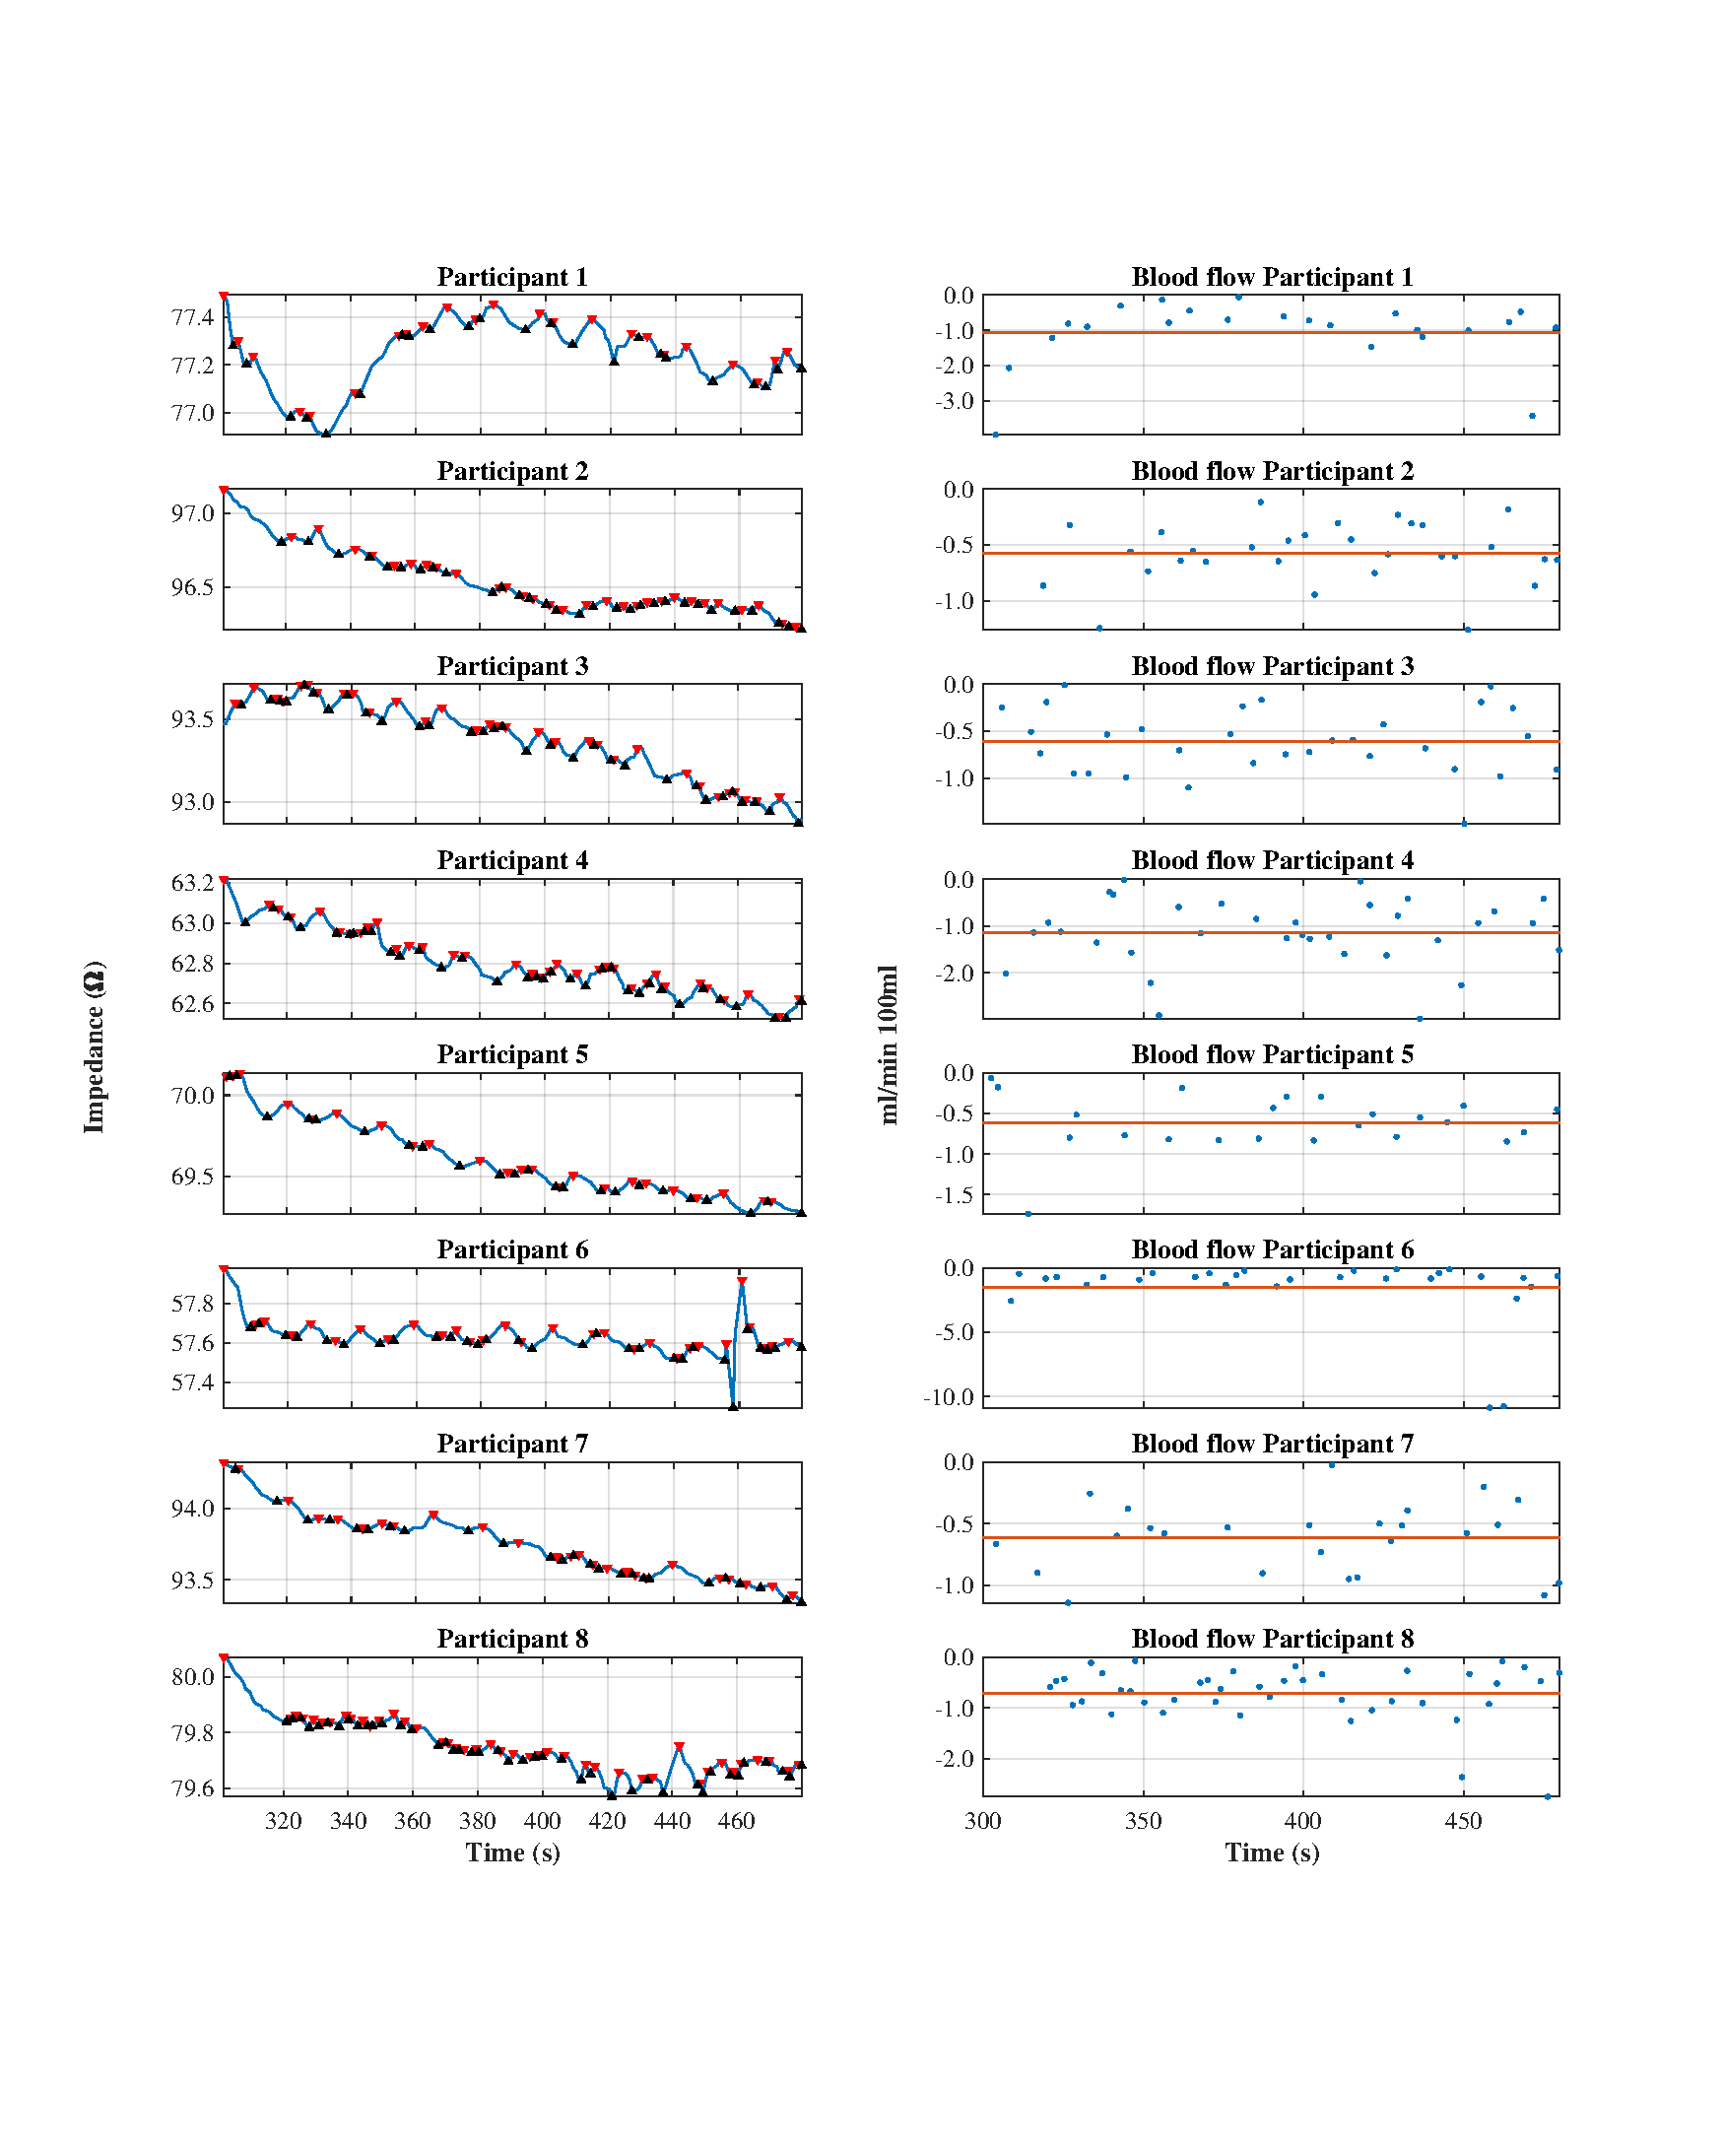
\includegraphics[width=\textwidth,height=\textheight,keepaspectratio,trim={0.5cm 0.5cm 2cm 2cm},clip]{figure12}    
	\caption{Blood flow calculated from venous occlusion plethysmography}
	\label{fig:blood_flow:venous_occlusion}
\end{figure}

%********************************** % Section 5.4.2 ******************************************
\subsection{Blood flow calculation during partial arterial occlusion}
\label{section5.4.2}
As reflected in \ref{section5.2.2}, there is a deeper slope in basal impedance during partial arterial occlusion compared to venous occlusion. Therefore, higher blood flow values are expected from the calculated data. The method used to estimate the blow was the same one utilised in the section \ref{section5.4.1}. The obtained signals were also affected by noise within the basal impedance, possibly caused by the respiratory action and muscle movement. In fact, during this part of the experiment, most participants felt uncomfortable feeling numbness in their arms. Therefore, they moved their arms during this section of the investigation which in part affected the quantification of blood flow.

The figure \ref{fig:blood_flow:arterial_occlusion} shows the calculation of the blood flow between the points of decreasing impedance. From a qualitative perspective, it can be observed that some signals do not show a decreasing linear trend. For example, participant 1 at the end of the test abruptly moved his arm causing a sudden change in impedance. As a result, the impedance at this point was far from the mean of the signal.

Another example of unexpected impedance change is the participant 4 and 8. In the first case, in the middle of the test, the impedance of the forearm tended to increase. However, this later began to decline as expected. In the second case, the movement of the arm can be observed after half of the test. As a result, there was a rapid acceleration of blood flow that is not in agreement with the average value of the signal.

By analysing the results summarised in the Table \ref{tbl:blood_flow:region4} the average blood flow of all the participants was \SI{-0.945}{\ml\per\min} $\pm$ \SI{0.224}{\ml\per\min 100\ml}. In general, there was an increment of \SI{9.52}{\percent} comapred to venous occlusion. 


\begin{table}[h]
	\caption{Statistics of the blood flow calculated during partial arterial occlusion. All the numbers are in blood flow units \si{\ml\per\min 100\ml}, except the column size that is the magnitude of sample.}
	\label{tbl:blood_flow:region4}
	\centering
	\begin{tabular}
		{
			l
			c
			c
			S[table-format=1.3]@{\,\( \pm \)\,}S[table-format=1.3] %Format for Z+-std 
			c
			c
		}
		\toprule
		& \multirow{2}{*}{\textbf{Size}} 
		& \textbf{Median} 
		& \multicolumn{2}{c}{\textbf{Mean}} 
		& \textbf{Max} & \textbf{Min} \\
		& 
		& \small{\si{[\ml/\min 100\ml]}} 
		& \multicolumn{2}{c}{\small{\si{[\ml/\min 100\ml]}}} 
		& \small{\si{[\ml/\min 100\ml]}} 
		& \small{\si{[\ml/\min 100\ml]}} \\\midrule
		Participant 1    &      24        &      -0.917    &      -1.118    &      1.090    &      -0.105    &      -5.238    \\ 
		Participant 2    &      27        &      -0.632    &      -0.950    &      0.996    &      -0.014    &      -4.821    \\ 
		Participant 3    &      27        &      -0.778    &      -0.966    &      0.736    &      -0.087    &      -3.546    \\ 
		Participant 4    &      35        &      -0.803    &      -1.184    &      1.129    &      -0.013    &      -5.462    \\ 
		Participant 5    &      22        &      -0.793    &      -0.725    &      0.292    &      -0.199    &      -1.250    \\ 
		Participant 6    &      28        &      -0.885    &      -0.952    &      0.695    &      -0.114    &      -2.628    \\ 
		Participant 7    &      25        &      -0.496    &      -0.524    &      0.350    &      -0.031    &      -1.498    \\ 
		Participant 8    &      26        &      -0.743    &      -1.141    &      1.170    &      -0.042    &      -4.708    \\ 
\bottomrule
	\end{tabular} 
\end{table}

\begin{figure}
	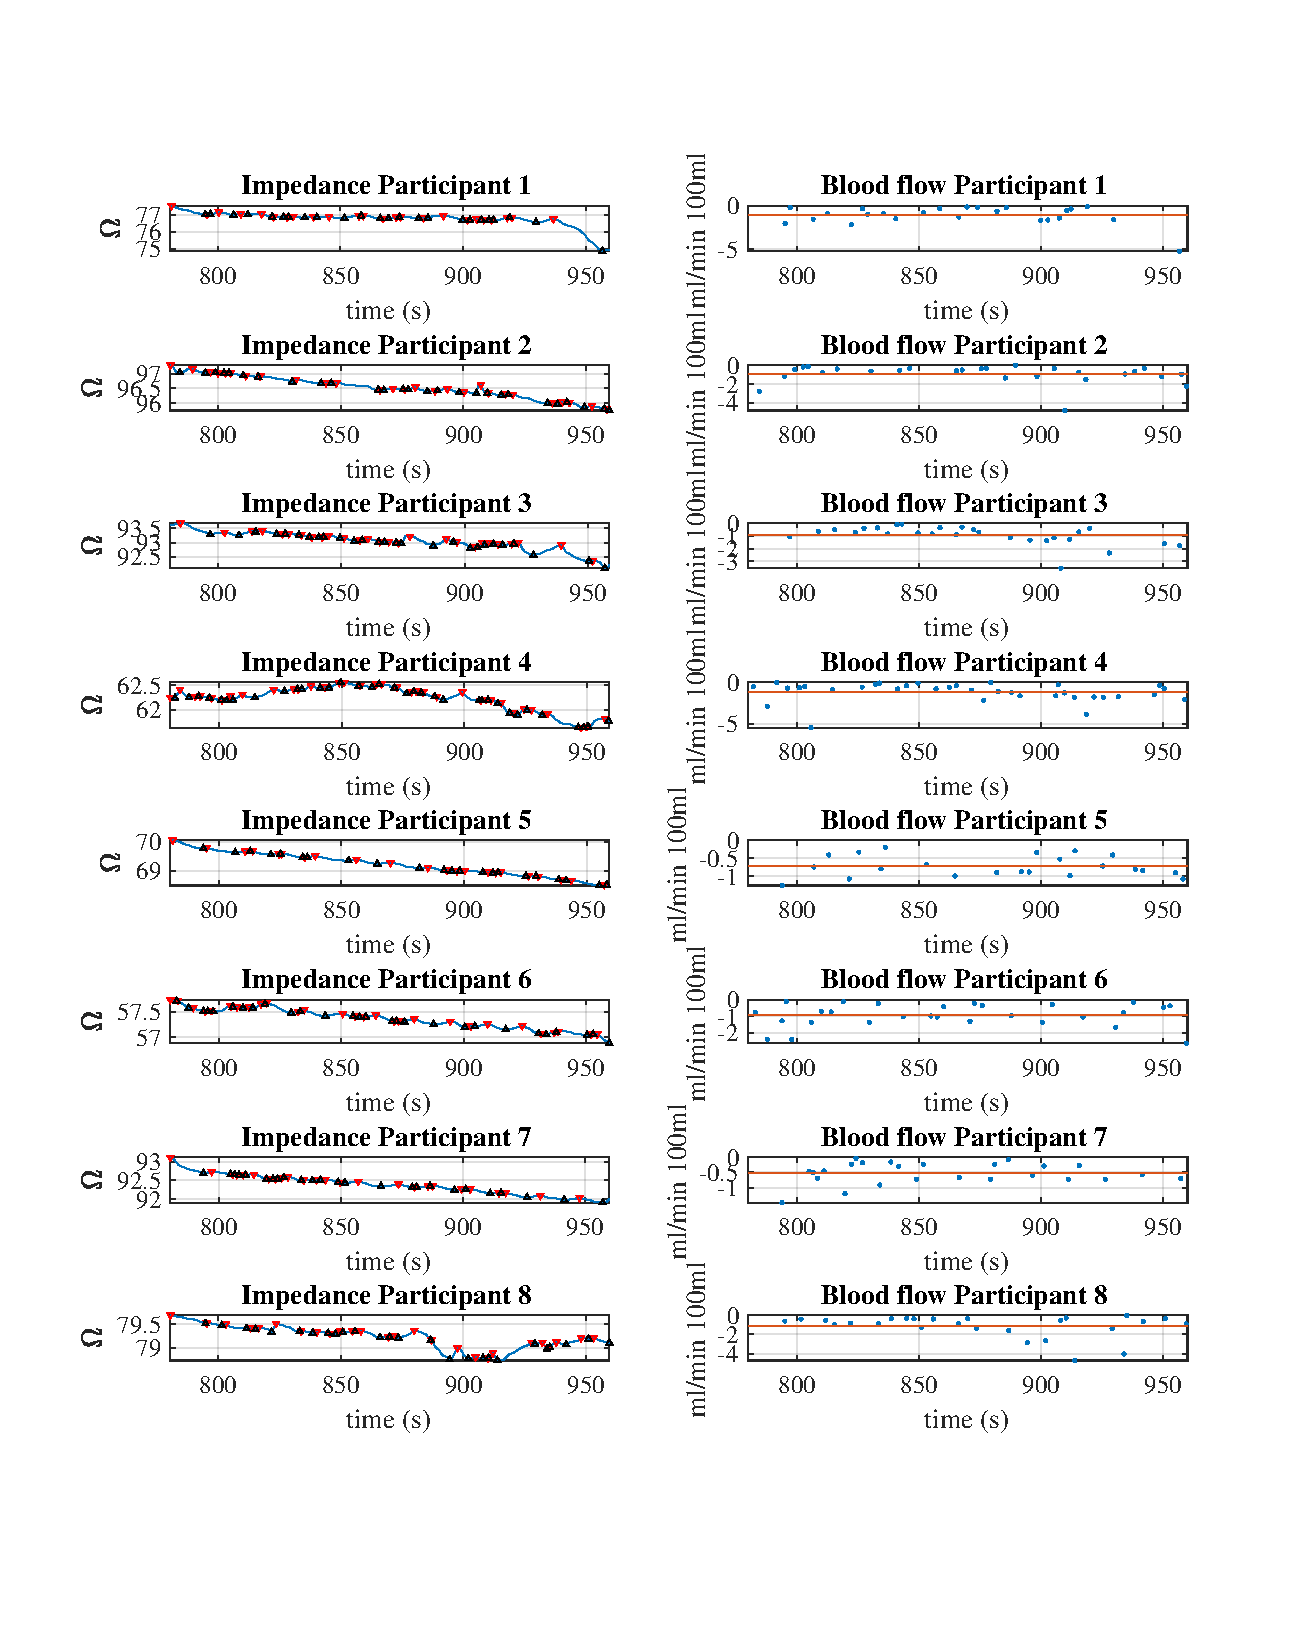
\includegraphics[width=\textwidth,height=\textheight,keepaspectratio,trim={0.5cm 0.5cm 2cm 2cm},clip]{figure13}    
	\caption{Blood flow calculated from partial arterial occlusion plethysmography}
	\label{fig:blood_flow:arterial_occlusion}
\end{figure}

%%********************************** % Section 5.4.3 ******************************************
\subsection{Comparative change of blood flow between venous and partial arterial}
\label{section5.4.3}
As it can be noticed from the qualitative analysis of the signals, the blow flow calculated during partial arterial occlusion points to be higher. 

\begin{figure*}[t!]
	\centering
	\begin{subfigure}[t]{0.5\textwidth}
		\centering
		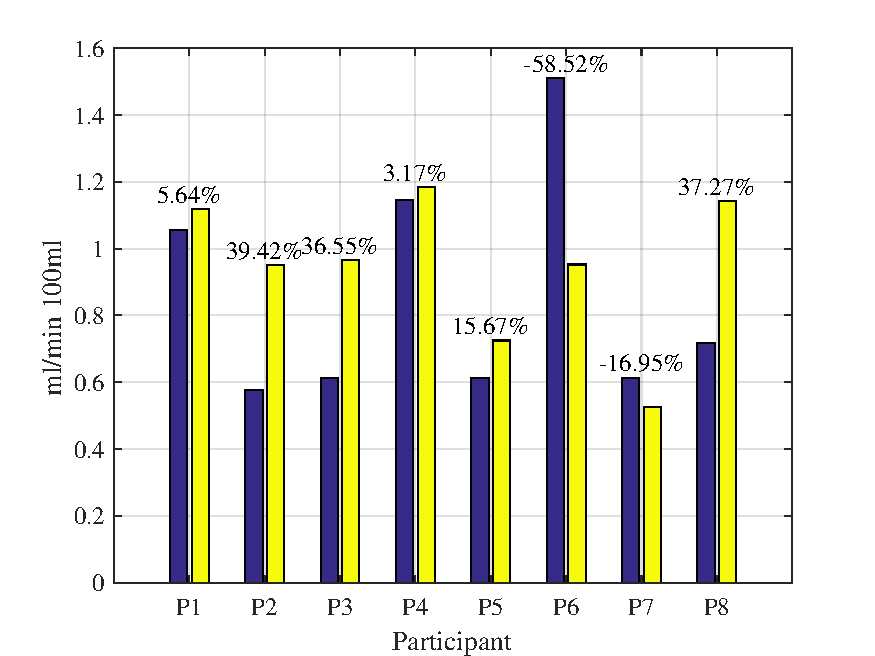
\includegraphics[height=6cm,keepaspectratio]{figure14a}    
		\caption{Comparison between mean venous occlusion and partial arterial occlusion. Ration of change showed as a percentage.}
		\label{fig:change_flow_mean}
	\end{subfigure}%
	~ 
	\begin{subfigure}[t]{0.5\textwidth}
		\centering
		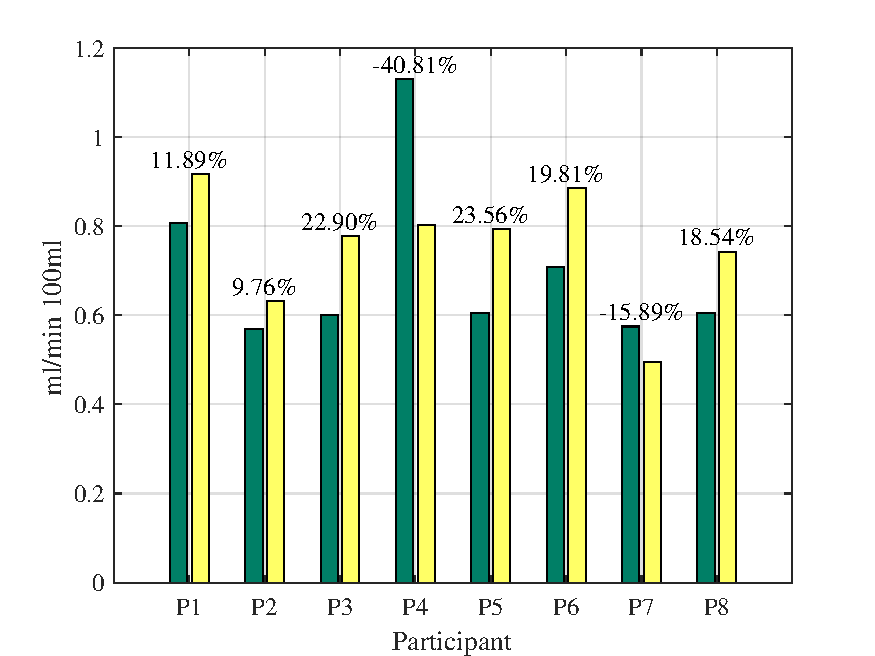
\includegraphics[height=6cm,keepaspectratio,keepaspectratio]{figure14b}    
		\caption{Comparison between median venous occlusion and partial arterial occlusion. Ration of change showed as a percentage.}
		\label{fig:change_flow_median}
	\end{subfigure}
	\caption{Change of blood flow between venous occlusion and partial arterial occlusion}
	\label{fig:iPG_flow_comparative}
\end{figure*}


%%********************************** % Section 5.5 ******************************************
\section{Blood flow calculation from plethysmography signal}
\label{section5.5}


%********************************** % Section 5.5.1 ******************************************
\subsection{Blood flow beat by beat during baseline}
\label{section5.5.1}

\subsection{Blood flow beat by beat during venous occlusion}
\label{section5.5.2}

\subsection{Blood flow beat by beat during partial arterial occlusion}
\label{section5.5.3}
